%  ========================================================================
%  Copyright (c) 1985 The University of Washington
%
%  Licensed under the Apache License, Version 2.0 (the "License");
%  you may not use this file except in compliance with the License.
%  You may obtain a copy of the License at
%
%      http://www.apache.org/licenses/LICENSE-2.0
%
%  Unless required by applicable law or agreed to in writing, software
%  distributed under the License is distributed on an "AS IS" BASIS,
%  WITHOUT WARRANTIES OR CONDITIONS OF ANY KIND, either express or implied.
%  See the License for the specific language governing permissions and
%  limitations under the License.
%  ========================================================================
%

% Documentation for University of Washington thesis LaTeX document class
% by Jim Fox
% fox@washington.edu
%
%    Revised 2020/02/24, added \caption()[]{} option.  No ToC.
%
%    Revised for version 2015/03/03 of uwthesis.cls
%    Revised, 2016/11/22, for cleanup of sample copyright and title pages
%
%    This document is contained in a single file ONLY because
%    I wanted to be able to distribute it easily.  A real thesis ought
%    to be contained on many files (e.g., one for each chapter, at least).
%
%    To help you identify the files and sections in this large file
%    I use the string '==========' to identify new files.
%
%    To help you ignore the unusual things I do with this sample document
%    I try to use the notation
%       
%    % --- sample stuff only -----
%    special stuff for my document, but you don't need it in your thesis
%    % --- end-of-sample-stuff ---


%    Printed in twoside style now that that's allowed
%
 
\documentclass [11pt, proquest] {uwthesis}[2020/02/24]
 
%
% The following line would print the thesis in a postscript font 

% \usepackage{natbib}
% \def\bibpreamble{\protect\addcontentsline{toc}{chapter}{Bibliography}}

\setcounter{tocdepth}{1}  % Print the chapter and sections to the toc

% ==========   Local defs and mods
%

\usepackage[utf8]{inputenc}
\usepackage{csquotes}
\usepackage[english]{babel}

\usepackage[style=authoryear,maxnames=99]{biblatex}[2014/06/25]
\addbibresource{uwthesis.bib}

\usepackage{graphicx}

\usepackage{siunitx}
\sisetup{per-mode=symbol-or-fraction}
\DeclareSIUnit\month{mo}
\DeclareSIUnit\millibar{mb}

\begin{document}
 
% ==========   Preliminary pages
%
% ( revised 2012 for electronic submission )
%

\prelimpages
 
%
% ----- copyright and title pages
%
\Title{Temporal Resolution and Process Coupling in Atmospheric Models}
\Author{Sean Patrick Santos}
\Year{2020}
\Program{Applied Mathematics}

\Chair{Christopher S. Bretherton}{Professor}{Department of Applied Mathematics and Department of Atmospheric Sciences}
\Signature{Peter M. Caldwell}
\Signature{Randall J. LeVeque}

\titlepage

\newpage

\copyrightpage

 
%
% ----- signature and quoteslip are gone
%

%
% ----- abstract
%


\setcounter{page}{-1}
\abstract{%
Insert abstract here
}
 
%
% ----- contents & etc.
%
\tableofcontents
\listoffigures
\listoftables
 
%
% ----- acknowledgments
%
\acknowledgments{% \vskip2pc
  % {\narrower\noindent
  Insert things here
  % \par}
}

%
% ----- dedication
%
\dedication{\begin{center}to my parents, for all their support, and to Buck, my lifeline through 2020\end{center}}

%
% end of the preliminary pages
 
 
 
%
% ==========      Text pages
%

\textpages
 
% ========== Chapter 1
 
\chapter{Introduction}

\chapter{The MG2 Microphysics}

\section{Timescales in MG2} \label{sec:mg2_timescales}

In this section we investigate the inherent timescales present in the MG2 code by calculating the eigenvalues of a numerically derived Jacobian.

\subsection{Methodology}

\subsubsection{Running MG2 as a Standalone Process}
\label{sec:MG2-standalone}

Within E3SM, MG2 and CLUBB are substepped together using a \SI{300}{\second} time step, which is both the default and maximum recommended time step for CLUBB. We can view the main role of MG2 as providing the average rates of change of MG2's ten state variables due to microphysical processes over a given time step.  We can evaluate how well MG2 answers this question without use of the full E3SM model, as long as we have a representative sample of atmospheric columns and a method for running MG2 outside of E3SM.

To obtain a sample of input columns, we ran a standard pre-industrial global E3SM simulation with $\sim$\SI{100}{\kilo\meter} atmospheric resolution (ne30\_ne30 grid) and prescribed sea surface temperature (compset F1850C5AV1C-04P2). The code used for this integration was a beta version (git hash 7a17edbe) which is structurally similar to the E3SMv1 release. Code modifications between this version and the release are not expected to make a difference for the results here. At the end of a five day run, we saved a ``snapshot'' of every column on the planet at the final time step, including every input used in the final call to MG2.

This provided us with a representative sampling of columns for a particular day in January, which is the basis for the analysis in the remainder of this paper. A larger or more varied sample of columns, taken over the course of a run lasting a year or more, would have some statistical differences, especially since such a sample would capture seasonal variation. However, since this sample causes MG2's most important processes to operate under a wide variety of conditions, we do not believe that broader sampling would affect our overall conclusions.

In order to run MG2 in isolation from the rest of the model, we used F2PY to create a Python interface and compiled MG2 and the interface into a stand-alone library. This library was used by a set of drivers to produce the MG2 stand-alone results in this paper.

We narrowed down the number of active processes to a subset of those in MG2 by implementing switches to disable two types of process. First, sedimentation was disabled in our runs. MG2's sedimentation runs sequentially after the state is updated by all other processes, and it uses an adaptive time step, smaller than that of MG2 as a whole, to satisfy its CFL condition. The numerical problems posed by the sedimentation are of a different character from those posed by the rest of MG2, and so we believe that it would be best to examine the sedimentation in a separate study. In fact, we consider the sedimentation to not be a microphysical process at all, but rather a dynamical process which happens to be packaged in MG2.

We do not believe that enabling sedimentation would affect the overall conclusions that we draw about the timescales relevant to resolved microphysics, especially since (as we shall see), these timescales are often too short to allow much sedimentation to occur. However, since the sedimentation time step can still be quite short for heavy rain ($<\SI{10}{\second}$), we do note that there may be benefits to coupling the sedimentation to MG2's other processes more frequently, though evaluating such a change is beyond the scope of this paper.

Since sedimentation is the (only) process in the MG2 microphysics that transports mass between levels, disabling sedimentation allowed us to view MG2 as a tool for solving an ODE in a collection of uncoupled grid cells, rather than as a tool for solving a 1D PDE on an atmospheric column. This provides two benefits:
\begin{enumerate}
\item All remaining processes have a well-defined and easily controlled time step, since only the sedimentation uses an adaptive time step.
\item If sedimentation was enabled with \num{72} vertical layers per column, then the state vector input to MG2 would be \num{720}-dimensional (given the \num{10}-dimensional state for each grid cell). With sedimentation disabled, MG2 operated on individual grid cells with a \num{10}-dimensional state in each one.
\end{enumerate}

Second, many ``instantaneous'' processes were disabled. Instantaneous processes are those processes which MG2 implements not by calculating an expected process rate, but by making an immediate adjustment from an state that is considered unstable or a violation of model assumptions, to a more stable or valid state. Usually such processes involve rapid changes of state, e.g. quickly melting snow that has fallen into a very warm grid cell.

We disabled these processes because we were interested in how the microphysical processes in MG2 are resolved, but instantaneous processes are by definition so fast that the model is not designed to resolve them in the first place. Furthermore, disabling the instantaneous processes removed any explicit dependence of the calculation on the time step size, which allowed the time step chosen during the Jacobian calculation to be chosen arbitrarily without impacting the results. Since these processes generally involve rapid melting/freezing of hydrometeors, we believe that our conclusions for warm cases, without significant ice physics, should not be affected by this change. However, when ice physics is present, MG2's resolved processes may be exposed to some states that are very different from those normally present in an E3SM run (e.g. large amounts of rain in very cold grid cells), so we should note that this modification results in MG2 effectively operating in a larger range of regimes than those normally present in a full model run. We take this behavior into account in interpreting results, so our conclusions are not erroneously affected by this modification.

One final change that was made to MG2 was to extract the calculation of precipitation area fraction from the main code, so that it was only calculated once per driver call. In conjunction with disabling sedimentation, this change was needed to allow MG2 to be run on individual grid cells rather than full columns, which greatly reduces computational cost. Furthermore, MG2's default precipitation area fraction calculation depends mostly on the cloud fraction calculated by CLUBB and is insensitive to changes in the state vector. As a result, forcing this variable to remain constant for short MG2 runs does not produce noticeably different results from allowing it to vary over time.

\subsubsection{Measuring Differences in MG2 States}

We often wanted to compare MG2 states in order to (a) establish whether MG2 is active enough to produce a final state that is very different from its input state, or (b) measure the magnitude of a change in MG2's output given a change in MG2's parameters. However, MG2's ten state variables include temperature, mass mixing ratios, and number concentrations, which have different units and orders of magnitude, so an isotropic norm such as the $L^2$ norm is ill-suited to represent the distance between MG2 states. One way to remedy this would be to use a set of constant weights to convert all variables to a common set of units; for instance, a difference in temperature could be converted to an approximate change in mass mixing ratio of liquid water that would be necessary to produce that change in temperature via evaporation/condensation.

A simpler approach is to focus solely on the mass mixing ratio terms in the state vector, from which we define a quantity called the total water mass difference ($D_w$). This is simply half of the $L^1$-norm of the water mass, or for two states labeled as $\mathbf{s_1}$ and $\mathbf{s_2}$:

\begin{eqnarray}
  D_w(\mathbf{s_1}, \mathbf{s_2}) &= \frac{\left|q_1 - q_2\right| + \left|q_{c1} - q_{c2}\right| + \left|q_{i1} - q_{i2}\right| +
    \left|q_{r1} - q_{r2}\right| + \left|q_{s1} - q_{s2}\right|}{2}
\end{eqnarray}

This value can be interpreted as the total amount of water that is in a different category between two states. For instance, consider if two states differ due to the evaporation of \SI{e-3}{\gram\per\kilo\gram} of rain. Then $q_r$ is reduced by \SI{e-3}{\gram\per\kilo\gram}, while $q$ is increased by the same amount; after dividing by $2$, we get $D_w = \SI{e-3}{\gram\per\kilo\gram}$.

The total water mass difference is arguably the most straightforward method for measuring the differences between MG2 outputs. Technically it does not account directly for differences in temperature, or at all for differences in number concentration. However, MG2 can only create changes in temperature via phase change, which will affect the mass mixing ratios, and in practice changes in number concentration will only occur in circumstances where processes that affect mass mixing ratio are also present. Differences in the overall MG2 state can therefore be distinguished by looking at mass mixing ratio alone.

\subsubsection{Jacobian Eigenvalue Calculation}

A standard method for analyzing the stability of a numerical method on a nonlinear problem is to linearize the system about a given state by calculating the Jacobian \parencite{RJL-FDM}. For a Jacobian with real eigenvalues, the eigenvectors represent those directions in which a perturbation to a system causes purely positive or negative feedback in the same direction, with the associated eigenvalues representing the sign and strength of that feedback. When an inappropriate numerical method is used, or the time step used with a given method is too long, the system's response to a perturbation will tend to rapidly amplify time integration errors, leading to instability. Accordingly, the stability of a linearized problem depends on the location of the eigenvalues of the Jacobian (multiplied by the time step) in the complex plane, and specifically on whether they fall in the stability region for a particular method (in our case, forward Euler).

Alternatively, one can think of the inverse of these eigenvalues as a set of timescales associated with the linearized system. In order to keep the system stable without depending on limiters or other artificial corrections to a given method, our time step must be sufficiently small compared to the smallest timescales derived from the Jacobian, so that the product of time step and eigenvalue lies within the method's stability region.

However, calculating this Jacobian presents some difficulty. The system of equations represented by MG2 is quite complex, and contains a large number of thresholds that adversely affect the smoothness of the process rates (e.g. the process rates are generally continuous, but not continuously differentiable, at the freezing point of water).

Rather than attempt to analytically differentiate MG2 around each point, we numerically calculated the Jacobian using the \emph{numdifftools} Python package. The specific method we used from this package is a second-order forward difference method, supplemented with one stage of Richardson extrapolation (so the resulting method is 3rd order accurate).

The use of a forward (rather than central) difference method was important. MG2 produces floating point exceptions when given negative concentrations, so we needed to use a one-sided method in order to numerically linearize about a state where any constituent has zero mass. Furthermore, by using a small linear change of variables, we could also ensure that this one-sided method does not use perturbed states that violate MG2's size limiters. Since MG2 enforces these limiters at several points throughout the code, any perturbation that leads to a state outside of the acceptable size ranges will result in an instantaneous adjustment back to a valid state, and these instantaneous adjustments are not of interest.

Since the Jacobian is a $\num{10} \times \num{10}$ matrix, finding its eigenvalues and eigenvectors was a negligible cost compared to the MG2 calls necessary to calculate the Jacobian in the first place. Thus we simply used SciPy's \emph{linalg.eig} (which wraps LAPACK calls that use the QR algorithm) for this calculation. The MG2 Jacobian almost always has a full set of eigenvectors when MG2 is active, though the Jacobian becomes defective when no hydrometeors are present. This appears to be because the process rates are completely insensitive to the temperature and humidity variables (rates are always zero in the absence of hydrometeors), but perturbations to the hydrometeor masses will result in temperature and humidity changes. This introduces asymmetric off-diagonal elements to the Jacobian that make it non-diagonalizable. We had no interest, however, in states where MG2 is inactive or nearly-inactive. We therefore only included cases where the process rates are sufficiently large, as defined by a total water mass difference threshold. Specifically, for an initial state $\mathbf{s_1}$ and a final state $\mathbf{s_2}$ we were only interested in columns where $(D_w(\mathbf{s_1}, \mathbf{s_2})/\Delta t) \ge \SI{e-7}{\gram\per\kilo\gram\per\second}$. Since most grid cells in the model have little to no condensate, this eliminated most of the total grid cells from consideration (\SI{79.7}{\percent}), which also significantly sped up calculations on the full sample.

The eigenvalues of the Jacobian are furthermore almost always real or have small imaginary parts, as shown in Figure \ref{complex-eigs}. This figure also shows that the few eigenvalues that have a large imaginary part also almost always fall within the region of absolute stability for the forward Euler method at a \SI{300}{\second} time step, unlike many of the purely real eigenvalues, which often have much larger magnitudes. We are therefore solely concerned with the real parts of these eigenvalues from this point forward.

\begin{figure}[ht]
  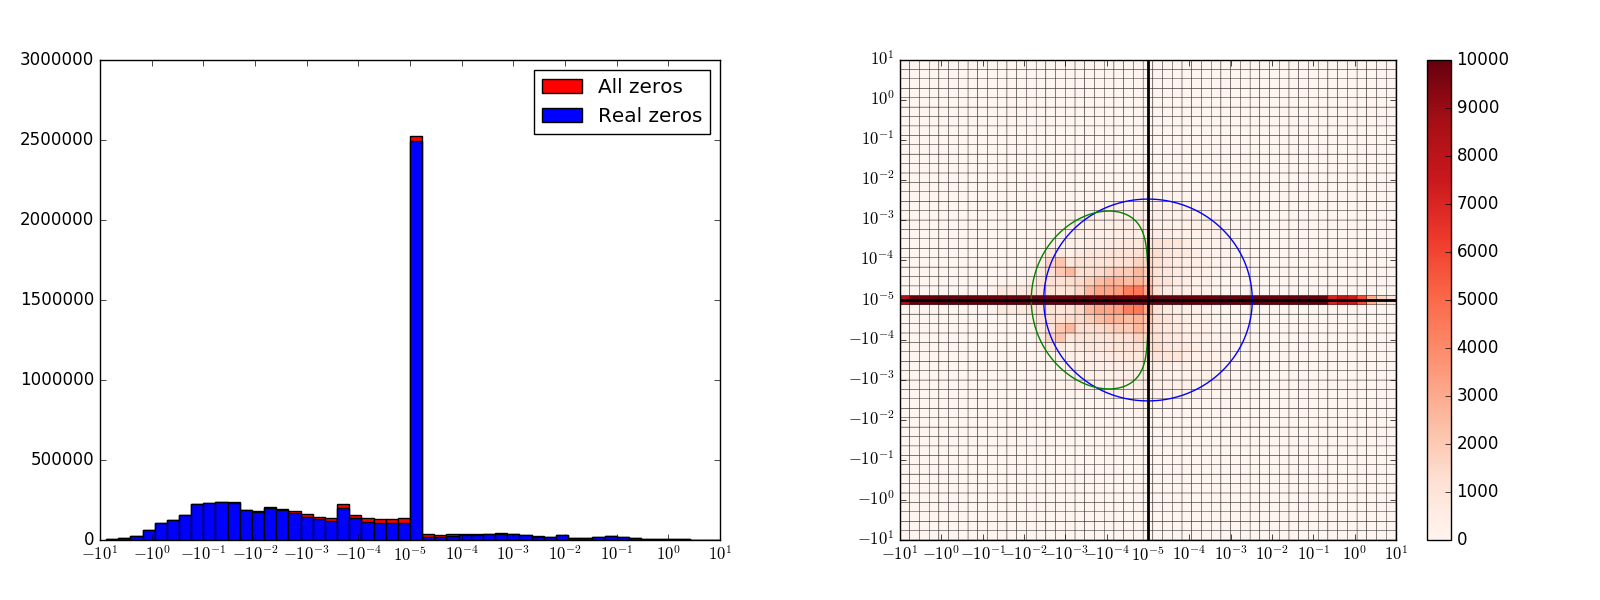
\includegraphics[width=6.5in]{./MG2Figure1.png}
  \caption{Graphs of complex eigenvalues, using a log scale. Eigenvalues with magnitude less than \SI{e-5}{\second} are placed at the origin. Left panel is a histogram comparing real zeros (taken to be those with $\le \SI{e-5}{\second^{-1}}$ imaginary part) with all zeros, showing that almost all eigenvalues are real. Figures \ref{neg-eig-hist} and \ref{pos-eig-hist} will show the negative and positive sections of this plot in more detail. Right panel shows distribution of eigenvalues in the complex plane, with a circle at $(\SI{300}{\second})^{-1}$ for comparison (blue), as well as the region of absolute stability for the Euler method (green). Real eigenvalues are apparent as a thick, dark line (i.e. exceeding the maximum of the colorscale) in this plot; this shows that real eigenvalues dominate.}
  \label{complex-eigs}
\end{figure}

\subsection{Results}

\label{sec:timescales-results}

\begin{figure}[ht]
  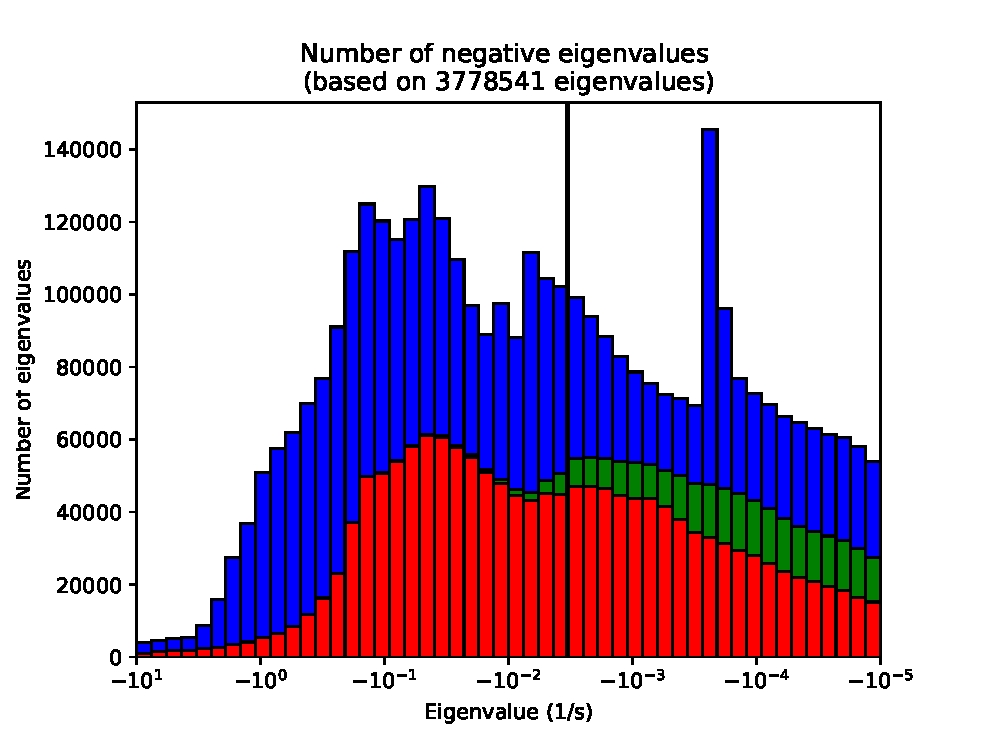
\includegraphics[width=6.5in]{./time_hist_all_values_neg.eps}
  \caption{Histogram of the real parts of the eigenvalues of MG2's Jacobian, focusing on negative eigenvalues. Red bars represent eigenvalues associated primarily with an active process (see Section \ref{sec:proc-timescales} for further details on this association). Green bars represent eigenvalues associated with at least one active process, but no ``primary'' process. Blue bars represent eigenvalues associated with inactive processes. A black line is placed at $(\SI{300}{\second})^{-1}$ for comparison with the MG2 time step.}
  \label{neg-eig-hist}
\end{figure}

\begin{figure}[ht]
  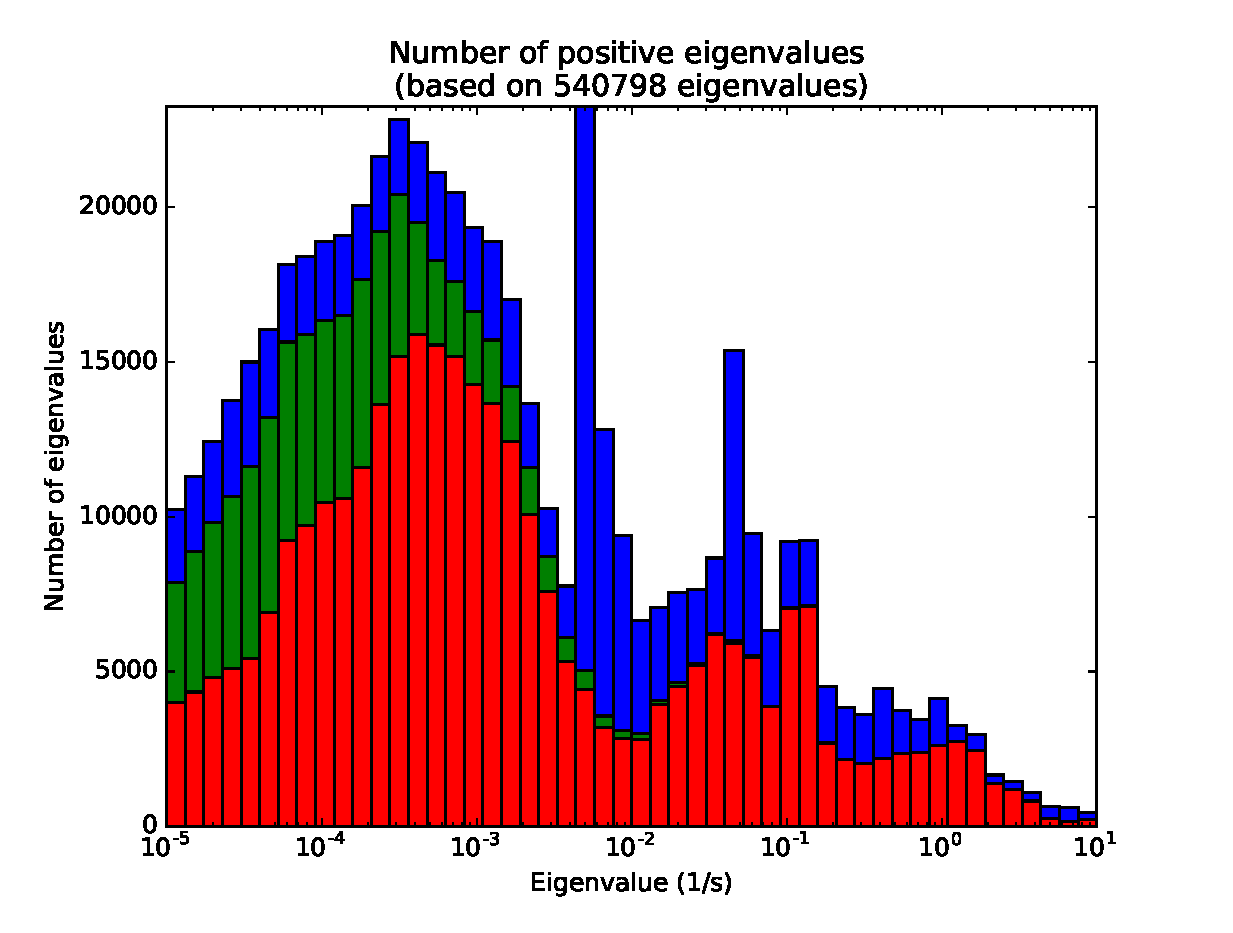
\includegraphics[width=6.5in]{./time_hist_all_values_pos.eps}
  \caption{Histogram of the real parts of the eigenvalues of MG2's Jacobian, focusing on positive eigenvalues. Red bars represent eigenvalues associated primarily with an active process (see Section \ref{sec:proc-timescales} for further details on this association). Green bars represent eigenvalues associated with at least one active process, but no ``primary'' process. Blue bars represent eigenvalues associated with inactive processes.}
  \label{pos-eig-hist}
\end{figure}

Figures \ref{neg-eig-hist} and \ref{pos-eig-hist} contain histograms of MG2's eigenvalues for grid cells above the \SI{e-7}{\gram\per\kilo\gram\per\second} cutoff. These eigenvalues are further categorized based on whether they are associated with active or inactive processes, where an active process is one that either affects water mass above a rate of \SI{e-7}{\gram\per\kilo\gram\per\second}, or affects a hydrometeor number above a rate of \SI{2.98e-3}{\per\kilo\gram\per\second}, which is equivalent to the rate of \SI{400}{\micro\meter} diameter rain particles that would have to be introduced to produce a mass change of \SI{e-7}{\gram\per\kilo\gram\per\second}. The details of how eigenvalues are associated with processes are explained in Section \ref{sec:proc-timescales}; we use association here just to indicate which eigenvalues are physically meaningful and which are akin to numerical noise. We can roughly divide these eigenvalues into five categories:

\begin{enumerate}
\item Eigenvalues associated with inactive processes (shown in blue). These eigenvalues are typically related to physics that is not active in a given regime, e.g. ice physics in a warm grid cell, so they are not as relevant to the numerics in practice.
\item Negative eigenvalues of magnitude greater than $(\SI{300}{\second})^{-1}$. These eigenvalues correspond to short-timescale processes, which have rates that may decay too rapidly for the default MG2 timescale to handle.
\item Negative eigenvalues of magnitude less than $(\SI{300}{\second})^{-1}$. These eigenvalues correspond to processes which MG2 is able to resolve, assuming roughly linear behavior of MG2.
\item Near-zero eigenvalues. These eigenvalues correspond either to extremely slow feedbacks within MG2, or to forbidden directions of motion in the phase space (particularly eigenvectors that are perpendicular to surfaces of constant energy or mass, since MG2's process rates must be tangent to such surfaces).
\item Positive eigenvalues. These eigenvalues correspond to eigenvalues of processes that are temporarily in a state of positive feedback (e.g. accretion produces larger raindrops, and those larger raindrops will be effective at accreting even more cloud water). Generally speaking, MG2 avoids instability from these processes due to its nonlinearity, since all MG2 processes ``use up'' some form of mass or number, and therefore will eventually slow down over time.
\end{enumerate}

In general we were most interested in dealing with the second case, the large negative eigenvalues, since these are common and correspond to cases where MG2's large timescale is likely to cause problems. Note that while the forward Euler method is absolutely stable up to eigenvalues of $(\SI{150}{\second})^{-1}$ at this time step, the $(\SI{300}{\second})^{-1}$ threshold is the point at which the method will produce a monotonic decay in the error. This is more relevant for avoiding negative mass concentrations, and therefore for avoiding triggering limiters that artificially constrain the process rates. Figure \ref{neg-eig-hist} shows that there are a great number of timescales that are not adequately resolved at MG's current time step (by this measure, even more than the number that do seem adequately resolved).

We also wanted to understand the nature of the positive eigenvalues, since these eigenvalues are always outside the region of stability for the forward Euler method (though this may not be as bad as it seems, as we discuss in Section \ref{sec:proc-assoc-results}).

In order to better interpret this result, however, we needed to associate the eigenvalues more closely with both specific sets of processes within MG2, and the physical conditions under which these eigenvalues arise. For instance, there may be cases where the model is formally unstable without limiters at a given time step, but in practice there is little difference between the resolved and limited behaviors.

\section{Connecting Timescales to Specific Processes} \label{sec:proc-timescales}

Documenting the timescales of MG2 processes was of inherent interest, but we were particularly interested in the finding that MG2 is often integrated using a $\Delta t$ which is too large to represent the processes it represents. Substepping all of MG2 in order to capture these timescales is not computationally feasible, but numerically accurate solutions may still be affordable if the need for substepping could be isolated to just a few processes.

\subsection{Methodology}
\subsubsection{Measuring Eigenvalue-to-Process Associations}

We sought to assign each eigenvalue from Sect. \ref{sec:mg2_timescales} to one or more of the MG2 processes listed in Table \ref{tab:processes}. Let us label the grid-cell output tendencies from applying MG2 to state $\mathbf{s}$ as $\mathbf{r} = \partial \mathbf{s}/\partial t$. The Jacobian $J_{\mathbf{r}}$ has $i,j$th entry $\partial r_i/\partial s_j$ where $r_i$ is the ith entry in $\mathbf{r}$ and $s_j$ is the $j$th entry in $\mathbf{s}$. As noted above, $J_{\mathbf{r}}$ is diagonalizable for the states that were of interest for us, so matrices of eigenvalues $\Lambda$ and eigenvectors $V$ exist such that $V \Lambda V^{-1} = J_{\mathbf{r}}$.

If we label the tendencies due to a particular process $p$ as $\mathbf{r}_p$, then $\Sigma_{p=1}^{P}\mathbf{r}_p = \mathbf{r}$. This leads directly to the identity
%-------------------------------------
\begin{eqnarray}
  \Lambda = V^{-1} (J_{\mathbf{r}}) V &= \Sigma_{p=1}^{P}V^{-1} (J_{\mathbf{r}_p}) V
\end{eqnarray}
%-------------------------------------
which is the heart of our association method. Now construct a matrix $\tilde{C}$ of dimensions $N$ (number of eigenvalues) by $P$ (number of processes to consider) whose $n,p$th entry $\tilde{C}_{np}$ is the $n$-th diagonal element of $V^{-1} (J_{\mathbf{r_p}})V$. Since it depends only on these diagonal elements, $\tilde{C}$ is independent of the scaling of the columns of $V$. Additionally,
%------------------------------------
\begin{eqnarray}
  \Sigma_{p=1}^{P}\tilde{C}_{np} &= \lambda_{n}
\end{eqnarray}
%-------------------------------------
so the $n$th row of $\tilde{C}$ represents the contributions from each process to the value of $\lambda_{n}$. The elements that contribute to a particular eigenvalue may be of different signs. Two large-magnitude values of $\tilde{C}_{np}$ may add to produce a larger $\lambda_{n}$, or they may partially cancel to produce a smaller $\lambda_{n}$. In either case, however, we would say that the largest magnitude values in $\tilde{C}$ have the most influence on the corresponding eigenvalues.

As a final step, normalize $\tilde{C}$ by taking the absolute value of each element, and by dividing each row by its $1$-norm, producing a new matrix $C$. Then each element of $C$ describes the fractional contribution of its column's process to its row's eigenvalue. If any element of $C$ is greater than \num{0.5} (our heuristic for whether at least \SI{50}{\percent} of an eigenvalue's magnitude can be attributed to a particular process), then we say that the eigenvalue for that row is \emph{primarily associated} with the process for that column. This is how the colors in Figures \ref{neg-eig-hist}-\ref{pos-eig-hist} are derived: the red bars count eigenvalues primarily associated with active processes, blue bars correspond to inactive processes, and green bars represent eigenvalues without a primary association. We are mainly concerned with large-magnitude eigenvalues, which almost all have a primary association with a particular process.

For purposes of this study, we treated the effects of MG2's size limiters as if they were a separate physical process. This was largely because MG2's state can become unrealistic or invalid if these limiters are disabled, so we were not able to disable them as we had with other instantaneous processes, and it was therefore necessary to account for their effects on MG2's state. Note also that these limiters are not applied purely for artificial, numerical reasons, since the maximum size limiters are also the means by which MG2 accounts for the spontaneous breakup of large particles, which is important especially for a reasonable treatment of precipitation.

\subsubsection{Correlation of Multiple Processes}

In addition to identifying processes associated with particular timescales, we wanted to identify tightly coupled processes. Such processes must be solved simultaneously or substepped together in order to obtain numerically accurate solutions. In addition, accounting for such coupling is needed in order to create useful conceptual models of microphysical behavior.

We hypothesized that processes that are tightly coupled in this way would be tend to be associated with the same eigenvalues. That is, while most eigenvalues have a single \emph{primary} association with another process, there are also large values of $C$ linking these eigenvalues to other processes, and we believed that this might signify cases where both processes must be solved together for accurate time integration.

To identify such possible sets of tightly coupled processes, we therefore first tallied the number of eigenvalues with primary associations to each process. We then looked at the average value of $C$ across all eigenvalues primarily associated with a given process. If, for instance, eigenvalues that are primarily associated with autoconversion also typically have strong association with accretion, then we would focus on autoconversion/accretion coupling for further study and optimization.

\subsection{Results}
\label{sec:proc-assoc-results}

We will first examine the association between positive eigenvalues and specific processes, shown in Figure \ref{process-2D-pos-eig}.

\begin{figure}[ht]
  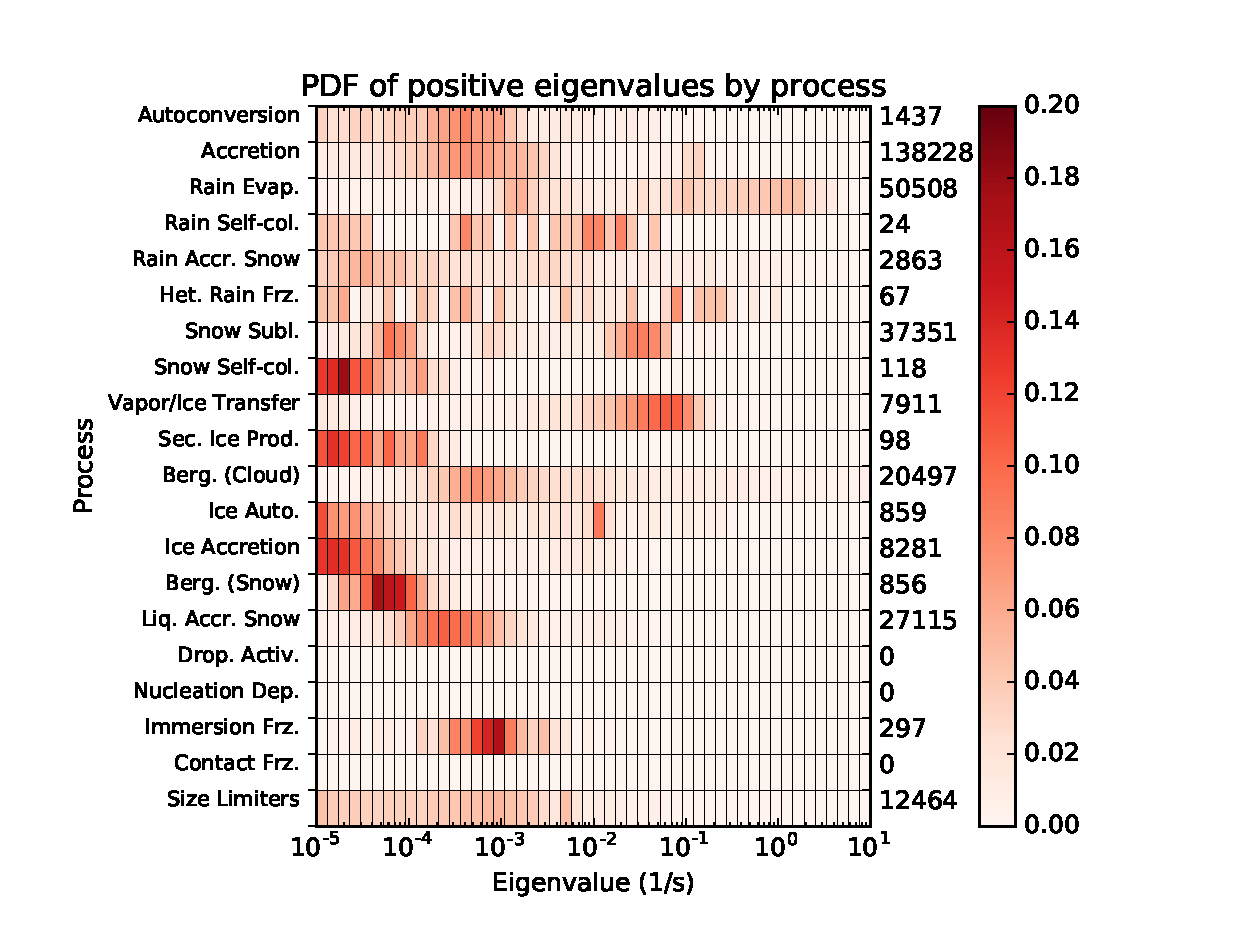
\includegraphics[width=6.5in]{./time_hist_process_2D_pos.eps}
  \caption{PDF of positive MG2 Jacobian eigenvalues, based on process primarily associated with each eigenvalue. Each row sums to \num{1}, except for processes with no associated positive eigenvalues. The right-hand y-axis label shows the number of positive eigenvalues associated with each process.}
  \label{process-2D-pos-eig}
\end{figure}

First, we found positive eigenvalues that are associated mainly with accretion-related processes (e.g. note the large number of eigenvalues associated with liquid accumulation onto rain and snow in Figure \ref{process-2D-pos-eig}). These eigenvalues are positive when the accumulating particles are small and few in number, since in this case the initial accretion increases the size of the particles, making them better at accumulating additional mass. In the long run, this is not a threat to the stability of the model, since eventually the accretion will begin to deplete the cloud, which will cause the rate of accretion to slow (see Figure \ref{accretion-regimes}). We will not examine this issue further here, but it should be noted that long time steps may delay the onset of heavy precipitation in these cases.

\begin{figure}[ht]
  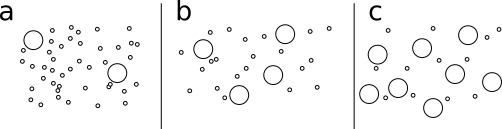
\includegraphics[width=6.5in]{./accretion_regimes.png}
  \caption{Diagram of accretion regimes. In case (a), the cloud mass is still much larger than the rain mass. As the rain accretes more liquid mass, it becomes more effective at accreting additional mass, so accretion experiences positive feedback. In case (c), the rain has already accreted most of the cloud, and further depletion of cloud mass slows the accretion rate, producing negative feedback. In case (b), cloud and rain mass are comparable, and these effects are in balance, producing only weak positive or negative feedback.}
  \label{accretion-regimes}
\end{figure}

Second, we found eigenvalues that are associated mainly with evaporation or sublimation (again in Figure \ref{process-2D-pos-eig}, there are large counts for rain evaporation, snow sublimation, and the Bergeron process). These eigenvalues are again positive mainly when the affected particles are small and few in number, as such particles rapidly evaporate when out-of-cloud. In such cases, the particle mass rapidly drops to zero, and the temporal resolution should not be relevant to the final state of the system.

Turning back to the negative eigenvalues, we wanted to examine the processes associated with the smallest timescales. As seen in Figure \ref{process-2D-neg-eig}, these processes are:

\begin{enumerate}
\item Accretion of cloud water by rain.
\item Rain evaporation.
\item Rain self-collection.
\item Snow sublimation.
\item Snow self-collection.
\item Vapor/Ice transfer.
\end{enumerate}

Other processes that were active with relatively short timescales include the Bergeron process and heterogeneous rain freezing, but we believe that the process rates are not being accurately calculated by our driver, and so we are less concerned about the apparent short timescales involved. The Bergeron process rate calculation is believed to be one of the least accurate parameterizations in MG2, primarily because it is poorly suited to the coarse spatial resolution used for GCMs, sometimes even resulting in a rate that is orders of magnitude too large \parencite{Tan2016,Zhang2019}. Reducing the time integration error is simply not a priority until this issue is addressed. As for the heterogeneous rain freezing, it is the process least likely to behave the same way in our driver as it does in E3SM, because we have disabled instantaneous freezing of rain, and the heterogeneous process should be expected to be more active to compensate.

The particular processes that we examined in more detail were rain evaporation, self-collection, and accretion of cloud water.  Partially this was because the purely liquid processes were easier to examine in isolation from the other physics, and partly this was because in practice the vapor/ice transfer was usually associated with small timescales only when the effect of this process was small anyway, so the error due to finite time resolution was small. In particular, sublimation of a small ice mass in relatively dry air can be quite rapid, but leads to the same behavior as given by the limited behavior, namely that the ice sublimates completely and rapidly.

We can also note that almost no eigenvalues are associated with the external processes, which is what we expect since these process' rates don't directly depend on the MG2 inputs, and only interact with MG2's physics due to being affected by the conservation limiters. In our data set, we found only three eigenvalues associated with contact freezing, a few thousand associated with immersion freezing, and none with nucleation deposition or droplet activation.

\begin{figure}[ht]
  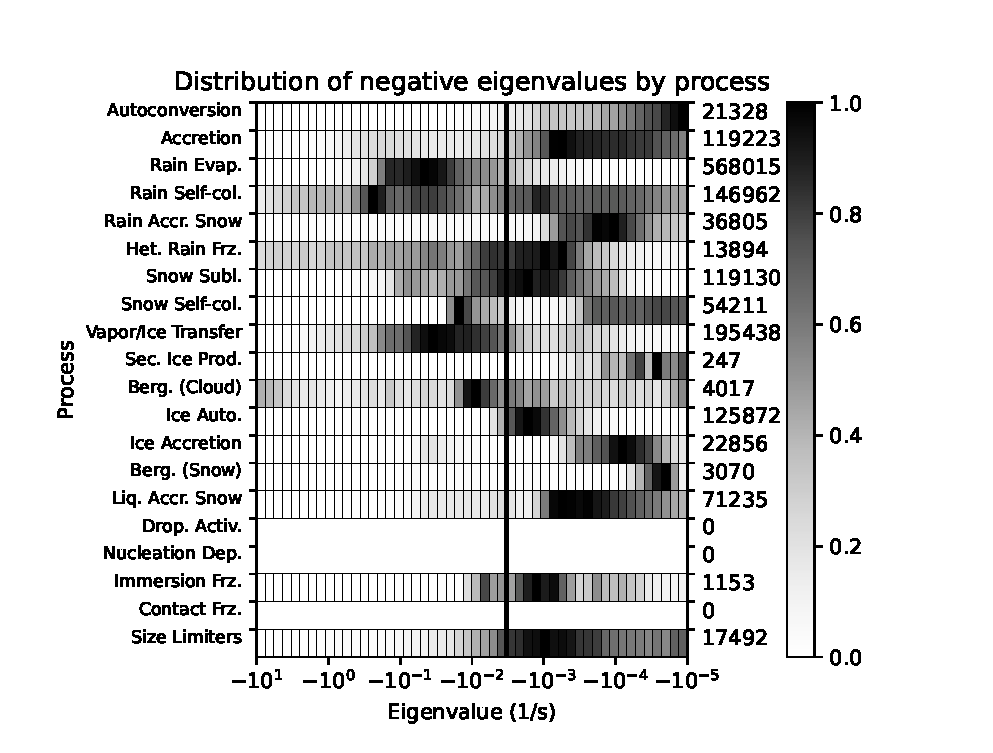
\includegraphics[width=6.5in]{./time_hist_process_2D_neg.eps}
  \caption{PDF of negative MG2 Jacobian eigenvalues, based on process primarily associated with each eigenvalue. Each row sums to \num{1}, except for processes with no associated negative eigenvalues.The right-hand y-axis label shows the number of negative eigenvalues associated with each process. A black line is placed at $(\SI{300}{\second})^{-1}$ for comparison with the MG2 time step.}
  \label{process-2D-neg-eig}
\end{figure}

Figure \ref{process-association} shows the degree to which different processes were associated with the same eigenvalues (and hence timescales). Looking at timescales associated primarily with the processes listed above, we found the following:

\begin{enumerate}
\item Accretion of cloud water by rain is associated with autoconversion.
\item Rain self-collection is strongly associated with rain evaporation.
\item The degree of association between ice processes is quite complex. In particular, vapor/ice transfer is associated with several processes, possibly because it is mildly active in a very large number of grid cells.
\end{enumerate}

\begin{figure}[ht]
  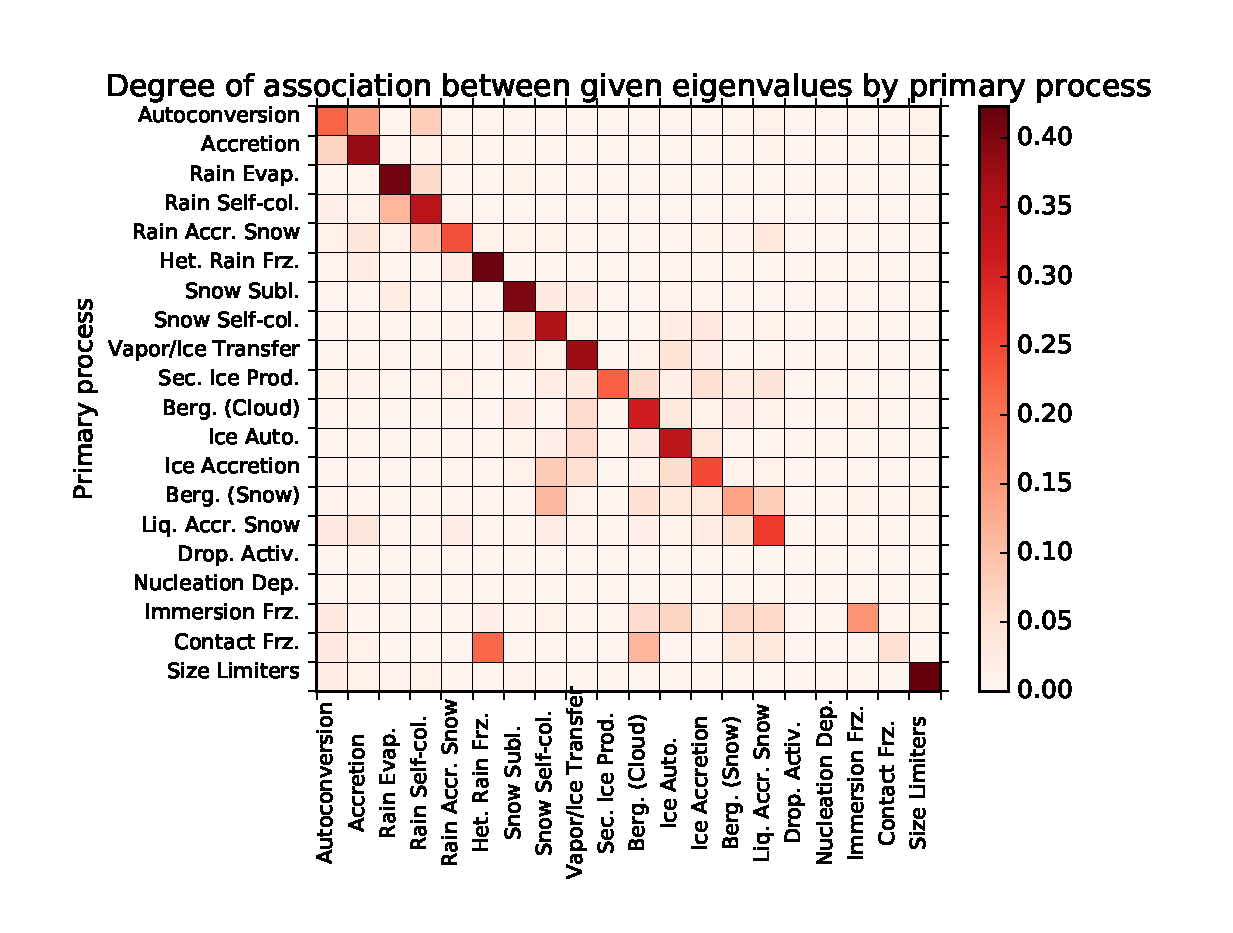
\includegraphics[width=6.5in]{./process_association.eps}
  \caption{Association between pairs of processes in MG2. Each row shows the average association index ($C$) for eigenvalues associated with a given primary process. That is, each row of the table shows the average value of a row of $C$ for eigenvalues primarily associated with the process shown on the left axis. By our definition of primary association, this means that all elements on the diagonal have values of at least \num{0.5}, so each entry on the diagonal has had its value reduced by \num{0.5} to fit in the same color range.}
  \label{process-association}
\end{figure}

As Figure \ref{process-2D-neg-eig} shows, the timescales associated with both liquid and ice autoconversion were relatively long. We therefore expected that the regime in which, say, liquid autoconversion and accretion interact most heavily would be different from the regime in which accretion by rain is associated with short timescales, and therefore we hypothesized that autoconversion should not require a short time step to adequately resolve, despite its association with accretion.

On the other hand, rain self-collection and evaporation were both primarily associated with the same short timescales, and so it appeared less likely that we could resolve rain-related processes without using a relatively short timescale for both.

\section{Decomposition by Weather Regime} \label{sec:regime}

Microphysics operates differently in different meteorological conditions. In particular, only a few microphysical processes are typically active at any particular point in space and time. Thus breaking cases down by weather regime can simplify the task of understanding model behavior. Such decomposition is also important because processes are likely to have different timescales depending on the weather regime they're in. For instance, the rate of accretion is fairly steady when rain and cloud mass are similar, but the accretion rate decreases rapidly when cloud becomes depleted, and the associated timescale is therefore much smaller in the latter case.

\subsection{Methodology}

We accomplished this decomposition by normalizing all process rates by typical values (so all processes were given approximately equal weight) and using a simple $k$-means algorithm to cluster grid cells based on process rates, so that we could treat the clusters as separate regimes.

We were interested in finding clusters containing qualitatively different, common types of behavior to examine in further detail, not in an objective categorization of all types of grid cells in the model. For this purpose we were content to use a degree of hand-tuning to determine both the total number of clusters and the scaling of process rates used in the clustering algorithm (for instance, reducing the effect of the Bergeron process). We iterated with changes to the cluster number and scaling until we found \num{10} clusters that had reasonably distinct process rates from one another.

Once this was accomplished, we could then look at the eigenvalues associated with the Jacobian for each cluster, in order to determine which regimes were likely to have short timescale behavior based on process rates alone.

\subsection{Results}

Table \ref{tab:clusters} gives a brief summary of the most active processes in each of these clusters, specifically those with mean rate above \SI{e-5}{\gram\per\kilo\gram\per\second} (or \SI{0.298}{\per\kilo\gram\per\second} for precipitation self-collection), as well as the number of grid points in each cluster. Note that these rates are \num{100} times greater than those used in Section \ref{sec:timescales-results}, since we are describing those processes that dominate the physics for each cluster, rather than those that simply have some appreciable activity. Note that cluster 0, which consists of generally clear-sky grid cells where no processes are particularly active, comprises the majority of our data set.

While the Bergeron process for cloud ice and heterogeneous rain freezing may seem quite large in many clusters, these should be disregarded for two reasons. Firstly, as noted in Section \ref{sec:proc-assoc-results}, these two processes are not likely to be well represented in our driver. For the Bergeron process, this is due to the low accuracy of MG2's representation of this process at the spatial resolutions used by GCMs. We believe that there will be little benefit to improving time integration of the Bergeron process until this more fundamental concern is addressed. As for the heterogeneous rain freezing, this process is likely affected by our standalone driver deviating from the behavior of MG2 within E3SM, in particular by the fact that the instantaneous rain freezing has been disabled. Secondly, our scaling deemphasized these processes, so they had the less impact on the clustering algorithm itself than the other MG2 processes.

\begin{table}
  \centering
  \scriptsize
  \begin{tabular}{|c|p{0.35\linewidth}|p{0.35\linewidth}|r|}
    \hline
    Index & Cluster Description & Active Processes & \# Grid Points \\
    \hline
    0 & MG2 mostly inactive. & Berg. (Cloud): \SI{1.03e-5}{\gram\per\kilo\gram\per\second} & \num{3404586} \\
    \hline
    1 & Ice cloud growth. & Berg. (Cloud): \SI{2.53e-2}{\gram\per\kilo\gram\per\second} \newline Vapor/Ice Transfer: \SI{3.58e-5}{\gram\per\kilo\gram\per\second} \newline Het. Rain Frz.: \SI{1.03e-5}{\gram\per\kilo\gram\per\second} & \num{2504} \\
    \hline
    2 & Snow accumulating rain and cloud liquid. & Het. Rain Frz.: \SI{1.11e-4}{\gram\per\kilo\gram\per\second} \newline Rain Accr. Snow: \SI{2.11e-5}{\gram\per\kilo\gram\per\second} \newline Liq. Accr. Snow: \SI{1.96e-5}{\gram\per\kilo\gram\per\second} \newline Rain Self-col.: \SI{2.57}{\per\kilo\gram\per\second} & \num{23854} \\
    \hline
    3 & Early/light rain production. & Autoconversion: \SI{1.59e-5}{\gram\per\kilo\gram\per\second} \newline Accretion: \SI{1.09e-5}{\gram\per\kilo\gram\per\second} \newline Rain Self-col.: \SI{16.16}{\per\kilo\gram\per\second} & \num{22378} \\
    \hline
    4 & Snow-producing cloud with out-of-cloud precipitation. & Het. Rain Frz.: \SI{1.26e-4}{\gram\per\kilo\gram\per\second} \newline Berg. (Cloud): \SI{1.00e-4}{\gram\per\kilo\gram\per\second} \newline Ice. Auto.: \SI{3.66e-5}{\gram\per\kilo\gram\per\second} \newline Snow Subl.: \SI{3.06e-5}{\gram\per\kilo\gram\per\second} \newline Rain Evap.: \SI{1.09e-5}{\gram\per\kilo\gram\per\second} \newline Snow Self-col.: \SI{1.40}{\per\kilo\gram\per\second} & \num{694} \\
    \hline
    5 & Out-of-cloud, mixed precipitation. & Berg. (Cloud): \SI{2.90e-4}{\gram\per\kilo\gram\per\second} \newline Rain Evap.: \SI{3.59e-5}{\gram\per\kilo\gram\per\second} \newline Snow Subl.: \SI{3.21e-5}{\gram\per\kilo\gram\per\second} \newline Rain Self-col.: \SI{0.619}{\per\kilo\gram\per\second} & \num{5456} \\
    \hline
    6 & Late/heavy rain production. & Accretion: \SI{3.80e-5}{\gram\per\kilo\gram\per\second} \newline Autoconversion: \SI{1.15e-5}{\gram\per\kilo\gram\per\second} \newline Rain Self-col.: \SI{47.46}{\per\kilo\gram\per\second} & \num{5404} \\
    \hline
    7 & Heavy rain in a concentrated area. & Rain Evap.: \SI{1.25e-4}{\gram\per\kilo\gram\per\second} \newline Rain Self-col.: \SI{511}{\per\kilo\gram\per\second} & \num{849} \\
    \hline
    8 & Snow-producing cloud with all precipitation in cloud. & Het. Rain Frz.: \SI{3.63e-4}{\gram\per\kilo\gram\per\second} \newline Berg. (Cloud): \SI{2.73e-5}{\gram\per\kilo\gram\per\second} \newline Liq. Accr. Snow: \SI{1.37e-5}{\gram\per\kilo\gram\per\second} \newline Ice. Auto.: \SI{1.00e-5}{\gram\per\kilo\gram\per\second} \newline Rain Self-col.: \SI{1.00}{\per\kilo\gram\per\second} \newline Snow Self-col.: \SI{0.535}{\per\kilo\gram\per\second} & \num{4579} \\
    \hline
    9 & Rain over a broad area. & Rain Evap.: \SI{3.48e-4}{\gram\per\kilo\gram\per\second} \newline Rain Self-col.: \SI{44.5}{\per\kilo\gram\per\second} & \num{29040} \\
    \hline
  \end{tabular}
  \caption{Description of clusters found through k-means algorithm}
  \label{tab:clusters}
\end{table}

Note that this provides another, simpler way to look at associations between processes. Looking again at liquid autoconversion and accretion, we see that these two processes are active together in clusters 3 and 6, but that the rate of accretion is much larger in cluster 6. We can then look at the eigenvalues of the Jacobian based on cluster, which is shown in Figure \ref{cluster-2D-neg-eig}. Unsurprisingly, the negative eigenvalues are much larger in cluster 6, implying that the short timescales are associated with the heavy accretion present in cells with a relatively large in-cloud rain mass.

\begin{figure}[ht]
  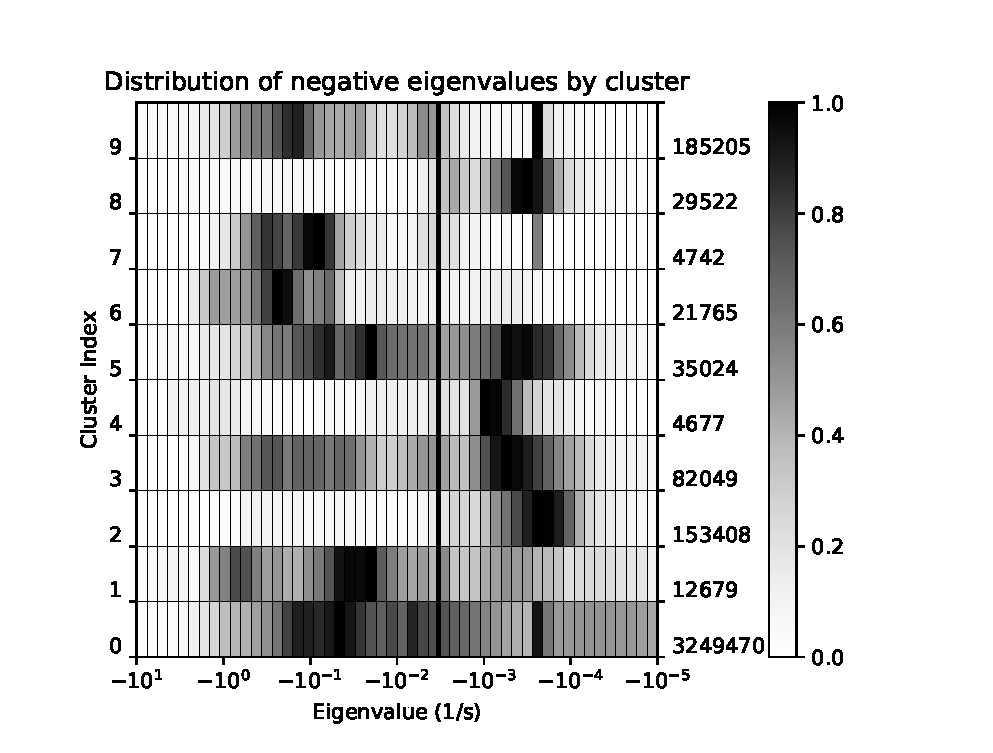
\includegraphics[width=6.5in]{./time_hist_cluster_2D_neg.eps}
  \caption{PDF of negative MG2 Jacobian eigenvalues, based on cluster of grid cell where the eigenvalue was calculated. The right-hand y-axis label shows the number of eigenvalues plotted for grid points in each cluster.}
  \label{cluster-2D-neg-eig}
\end{figure}

Similarly, we can use other clusters to examine other sets of short timescale processes. Cluster 1 would the best test case for short timescales associated with the Bergeron process and ice deposition (if the Bergeron parameterization was made more accurate). Rain evaporation and self-collection are both active and associated with short timescales in clusters 7 and 9.

\section{Impact of Shorter time steps} \label{sec:impact}

In the previous sections we identified processes and combinations of processes that evolve much more rapidly than the default model step. In this section we test whether accurately resolving those processes has a big impact on model behavior.

\subsection{Methodology}

In this section, we focus on two clusters, each associated with a set of processes that we believed would change considerably if substepped so as to resolve their behavior:

\begin{enumerate}
\item Grid cells with large rain self-collection and evaporation rates, corresponding to heavy out-of-cloud rain. (Cluster 9)
\item Grid cells with large accretion rates and moderate autoconversion rates, corresponding to heavy in-cloud rain. (Cluster 6, filtered to remove grid cells with any ice process rate or rain evaporation rate above \SI{e-7}{\gram\per\kilo\gram\per\second})
\end{enumerate}

The subsampling of cluster 6 was necessary to remove cases where accretion and autoconversion were not the only active processes. This was necessary for two reasons. Firstly, the clustering algorithm alone did not perfectly separate those grid cells with only rain production from grid cells that combined rain production with evaporation/sublimation of precipitation falling from above. Secondly, in some grid cells, especially at large time step sizes, the cloud liquid is turned completely to rain. If all cloud mass is removed from a grid cell, MG2 no longer considers the fraction of the grid cell that was occupied by the cloud to be saturated, and rain evaporation turns on. Since we were interested in the effect of substepping on autoconversion and accretion specifically, we removed grid cells where this occurred from this portion of the study. It should be noted that rain self-collection is also active in cluster 6. However, autoconversion and accretion within MG2 are not functions of the rain number, so it is not necessary to account for rain self-collection to accurately represent these processes.

For each of these cases, we produced modified versions of the MG2 standalone driver from Section \ref{sec:MG2-standalone}, which allowed these processes to be run at a smaller time step using the forward Euler method. For instance, for heavy in-cloud rain, autoconversion and accretion were substepped inside a nested series of loops, so that it was possible to adjust the time step of each independently of MG2 as a whole. If both processes were run at a finer time step, it was also possible to independently adjust the coupling frequency. By adjusting these time steps, it was possible to determine which processes needed to be better resolved to improve MG2's accuracy, and which were less relevant.

In order to assess the accuracy of these substepped simulations, it was necessary to decide upon both a measure of error, and a ``converged'' result for comparison. To measure the error in each grid cell, we used the total water mass difference defined above ($D_w$), which for Cluster 9 was effectively identical to the evaporation rate due to the absence of other influences (recall that $D_w$ only accounts for the error in water mass, not hydrometeor number). The converged result was chosen by using MG2 run at a very fine time step of \SI{75/512}{\second}, which is \num{1/2048} of the normal MG2 time step of \SI{300}{\second}. Using a power of two in this way is convenient for convergence studies, where the time step can be progressively halved to provide results that are closer and closer to converged.

Note that for the forward Euler method, the time integration error should be proportional to the time step (first order convergence). However, this is typically expected to hold only for short enough time steps, and in particular there is no guarantee that this will hold when the method is kept stable by limiters rather than because the method is absolutely stable at a given time step. Generally, there is little point in reducing the time step size if doing so does not much improve the accuracy, so when the time step for a process is reduced, we generally hope to reach the regime where first order convergence holds, as a bare minimum.

\subsection{Results}

We hypothesized that for the grid cells with large rain evaporation, there would be a noticeable benefit from substepping rain self-collection as well, since our Jacobian-based analysis associates these two processes with the same short timescales.

Since these timescales are typically around \SI{20}{\second}, we also expect to see roughly first-order convergence for time steps shorter than this, but not for larger time step sizes, because for larger time steps this method (or rather, its linearization around a typical state) is not stable on this problem. The model therefore becomes increasingly dependent on limiters for longer time steps.

The actual evaporation/self-collection results are shown in Figure \ref{convergence-evap-scol}. For comparison, note that the mean evaporation rate in this cluster is about \SI{1.82e-4}{\gram\per\kilo\gram\per\second}, so the mean error at a \SI{300}{\second} time step is an appreciable fraction of the evaporation rate itself. Substepping evaporation by itself is indeed much less effective than substepping both processes together. The self-collection of raindrops is a very fast process in MG2, and accounting for this considerably reduces the rate of evaporation. In particular, for grid points in cluster 9, the self-collection causes rain drops to reach the maximum allowed size in less than \SI{300}{\second}, meaning that unless processes like rain evaporation are coupled at a smaller timescale, the particle size is effectively determined by the size limiter, not the details of the self-collection itself. This is one reason it is unsurprising that we see sub-linear convergence at larger time step sizes.

\begin{figure}[ht]
  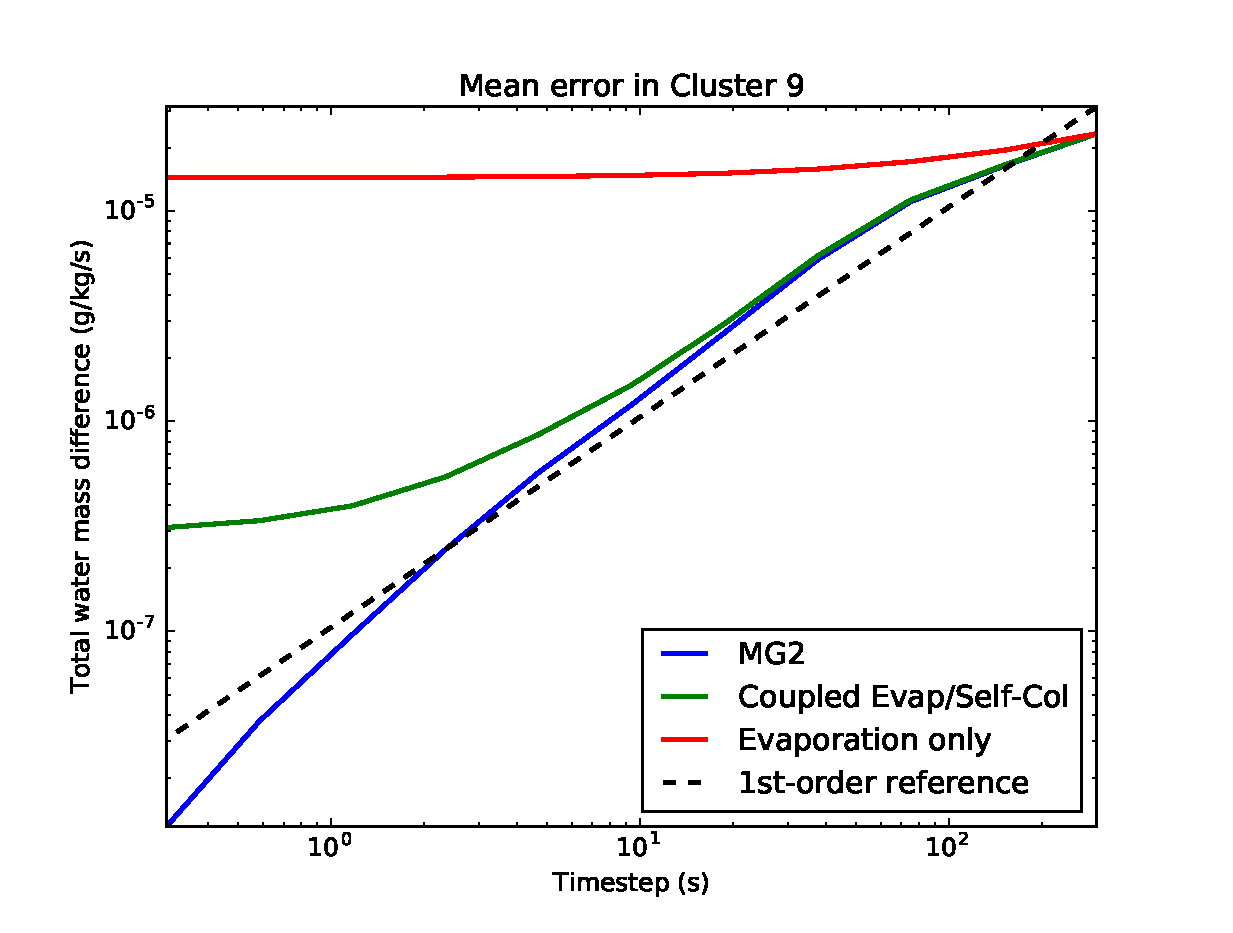
\includegraphics[width=6.5in]{./substep_convergence_mean_c9.eps}
  \caption{Convergence plot for mean error in cluster 9 grid cells under different substepping strategies for rain evaporation and self-collection. Runs substepping all of MG2 are shown in blue. Runs substepping evaporation and self-collection together, with total MG2 time step held fixed at \SI{300}{\second}, are shown in green. Substepping evaporation alone, with all other processes at \SI{300}{\second}, shown in red. The dotted reference line has slope \num{1}.}
  \label{convergence-evap-scol}
\end{figure}

Furthermore, the rate of convergence of the model becomes first order below a time step size of roughly \SIrange{30}{60}{\second}, both when all of MG2 is substepped and when only these two processes are substepped together. In fact, it appears faster than first order when all of MG2 is substepped. This may be due to the fact that our ``resolved'' result is the \SI{75/512}{\second} result, and this causes some underestimation of the error in the leftmost few points on the graph. At very short time steps, the error levels off when substepping only evaporation and self-collection due to small contributions from other, non-substepped processes in the grid cell (e.g. small amounts of cloud are present, causing some accretion, though the average accretion rate in this cluster is orders of magnitude less than the evaporation rate).

For grid cells dominated by accretion and autoconversion, we expected the effect of substepping accretion to matter much more than that of autoconversion, since autoconversion is associated almost exclusively with timescales longer than the maximum MG2 step size of \SI{300}{\second}. Similar to the evaporation case, we expected that first-order convergence would occur only for timescales shorter than about \SI{5}{\second}.

Figure \ref{convergence-accr-auto} shows the results of this substepping of accretion and autoconversion in cluster 6. Accretion rates are \SI{1.13e-4}{\gram\per\kilo\gram\per\second}, so the error is again comparable to the accretion rate itself. Substepping autoconversion alone is ineffective for reducing the error. Substepping the accretion, however, can cut the errors by more than an order of magnitude, while substepping autoconversion as well improves the error by only another factor of \num{2}.

\begin{figure}[ht]
  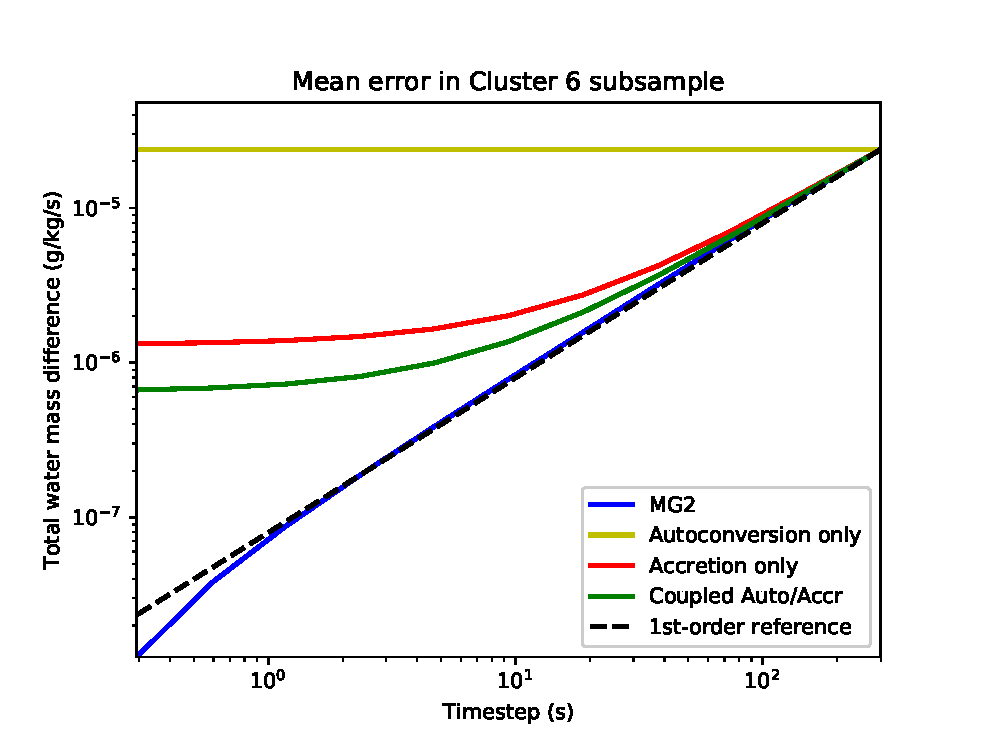
\includegraphics[width=6.5in]{./substep_convergence_mean_c6.eps}
  \caption{Convergence plot for mean error in cluster 6 subsample under different substepping strategies for accretion and autoconversion. Runs substepping all of MG2 are shown in blue. Runs substepping accretion and autoconversion together, with total MG2 time step held fixed at \SI{300}{\second}, are shown in green. Substepping accretion alone is shown in red, and substepping autoconversion alone is shown in yellow. The dotted reference line has slope \num{1}.}
  \label{convergence-accr-auto}
\end{figure}

However, we find, somewhat surprisingly, a near-perfect first-order convergence when substepping these processes, even out to \SI{300}{\second}. Note, again, the much smaller timescales in cluster 6 shown in Figure \ref{cluster-2D-neg-eig}, which would seem to suggest that this time step would produce instability, not linear convergence.

We came to suspect that by subsampling cluster 6, we had removed the grid points with the shortest timescales. There are three possible reasons this could happen. Firstly, the grid points with active ice processes could have been the grid points disproportionately associated with the shortest associated timescales. Secondly, the grid points with no ice processes but some evaporation at the beginning of the time step could be responsible, since some grid cells with out-of-cloud precipitation were included. Finally, some grid points could have no rain evaporation at the beginning of the time step, but develop rain evaporation over the course of a time step. In these grid points, at the beginning of the time step, all rain is considered to be inside the cloud, and no evaporation occurs. However, if the cloud is depleted to a concentration of less than \SI{e-3}{\gram\per\kilo\gram}, MG2 ignores the cloud area and assumes that all precipitation is outside the cloud, and therefore can evaporate.

Figure \ref{eig-c6-subsample} shows the results of our investigation. We find that our subsample did in fact include mostly points associated with long timescales, and excluded the majority of shorter timescales. Furthermore, the majority of points in cluster 6, especially those associated with short timescales, were points that started with no active evaporation or ice processes, but which ended up depleting enough cloud to cause MG2's evaporation process to switch on.

\begin{figure}[ht]
  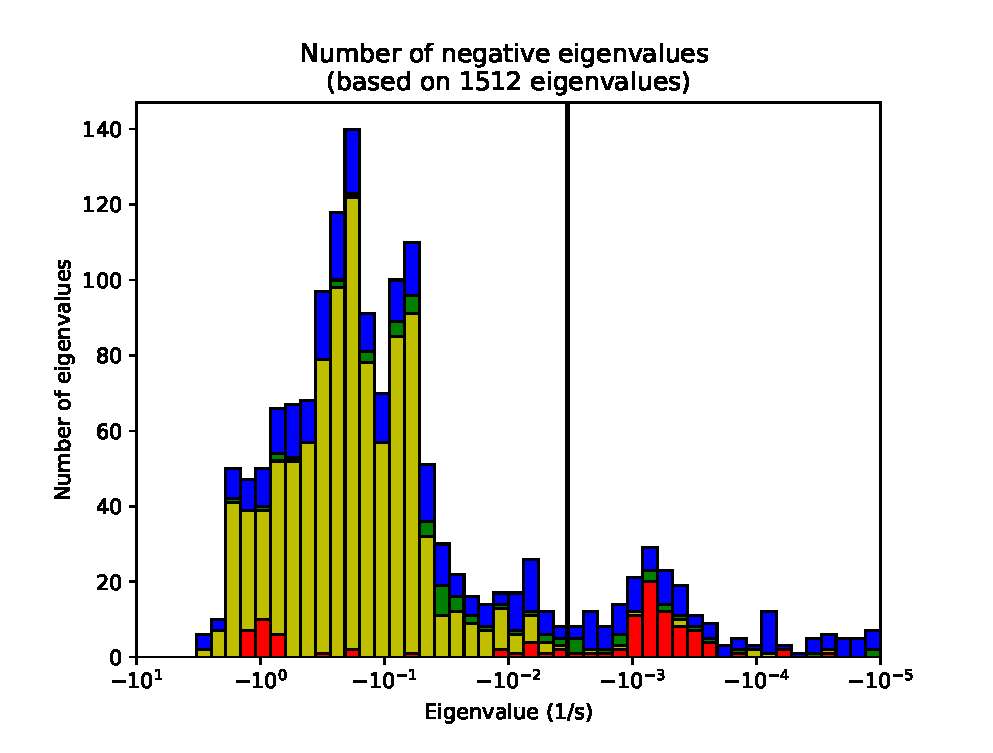
\includegraphics[width=6.5in]{./time_hist_all_values_neg_c6_subsample.eps}
  \caption{Histogram of negative eigenvalues in cluster 6. Blue bars correspond to eigenvalues at grid points excluded from the subsample due to having active ice processes (\num{647} grid points). Green bars correspond to grid points excluded due to having active rain evaporation at the beginning of the time step (\num{118} grid points). Yellow bars correspond to the grid points excluded due to developing rain evaporation over the course of a time step (\num{3796} grid points). Red bars correspond to the grid points included in the subsample (\num{843} grid points). A black line is placed at $(\SI{300}{\second})^{-1}$ for comparison with the MG2 time step.}
  \label{eig-c6-subsample}
\end{figure}

Given this situation, we decided to use a second, broader subsample so as not to exclude points that develop rain evaporation. This corresponds to the yellow and red bars in Figure \ref{eig-c6-subsample}. For this broader subsample, substepping accretion and autoconversion alone would probably not be sufficient to adequately represent the rain mass overall, since rain evaporation also becomes an important process. However, we might hope that substepping accretion and autoconversion together would at least reduce error in the rain production rate, especially since most evaporation should occur after the cloud is depleted, when the accretion should be slowing down.

Unfortunately, this is not the case, as Figure \ref{convergence-accr-auto2} shows. There is significant error in the rain production rate unless all rain-related processes are substepped together. We note that first-order convergence happens below a time step of about \SI{20}{\second}. Figure \ref{eig-c6-subsample} suggests that we might need an even smaller time step, but in practice, this does not seem to make much difference. This may be because these eigenvalues were calculated based on the conditions at the beginning of the time step. After some time has elapsed, the evaporation is turned on, while the self-collection is likely to cause the particles to reach maximum size, at which point the self-collection effectively turns off. This represents an important feature of MG2 not captured by our linear approach; if the time step is reduced, then different processes may activate at different times, and the timescales associated with active processes may also change over time.

\begin{figure}[ht]
  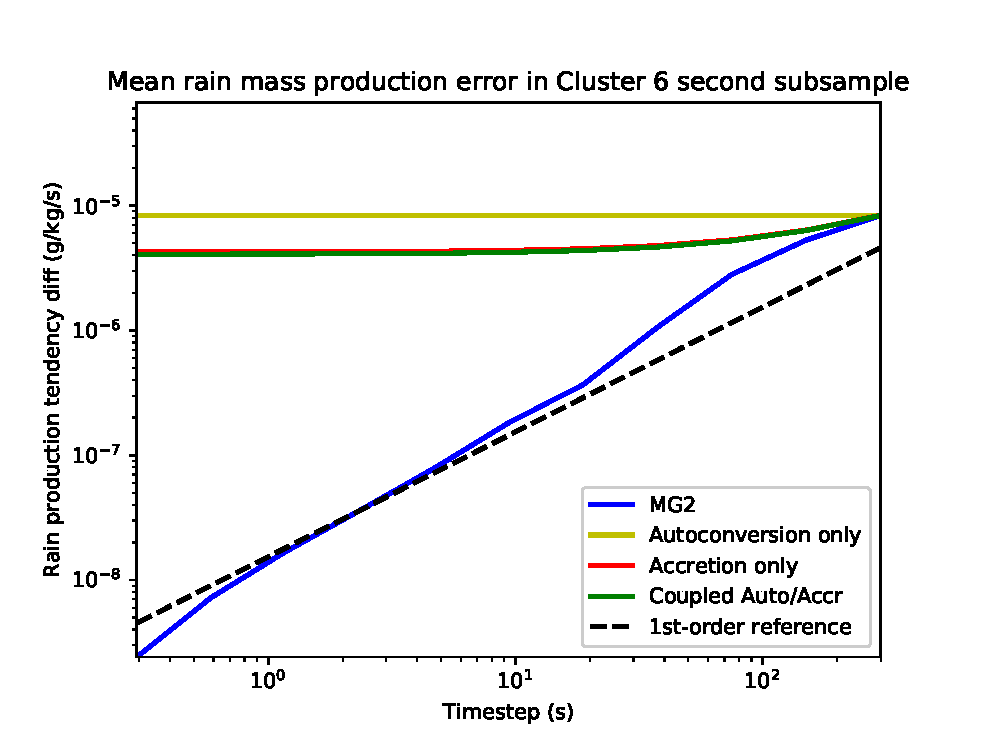
\includegraphics[width=6.5in]{./substep_convergence_prod_c6_initicefilter.eps}
  \caption{Convergence plot for mean error in second cluster 6 subsample, under different substepping strategies for accretion and autoconversion. Instead of the total water mass difference, only the rate of rain production (autoconversion+accretion) is plotted. Runs substepping all of MG2 are shown in blue. Runs substepping accretion and autoconversion together, with total MG2 time step held fixed at \SI{300}{\second}, are shown in green. Substepping accretion alone is shown in red, and substepping autoconversion alone is shown in yellow. The dotted reference line has slope \num{1}.}
  \label{convergence-accr-auto2}
\end{figure}

It is worth noting that all results in this section are broadly consistent with the prior literature in that they suggest a time step size of \SI{60}{\second} or below is necessary to reduce the error to within a few percent of the total process rate. Notably, in the case of rain evaporation, the error hardly improves until the time step is on the order of tens of seconds or lower.

\section{Discussion}

Our analysis of MG2, based on examining the eigenvalues of a numerically-derived Jacobian, shows that there are many situations where MG2 would appear to be unstable when using E3SM's forward Euler method at a \SI{300}{\second} time step. It is stable in practice due to nonlinearities in MG2, and especially due to the presence of limiters, but we would expect these limiters to reduce the accuracy with which E3SM solves the equations that MG2 is intended to implement.

This leads us to three concerns. First, is the time discretization error first-order, so that we can readily trade off increased computational cost for a proportional decrease in error? Or are there key unresolved timescales present in the system, so that the solutions we find at a \SI{300}{\second} time step are qualitatively different from the converged results? For instance, if certain process rates are typically constrained by limiters at long time steps, then modest improvements to the process rates will have little effect on the result, since both the original and ``improved'' process rates will be overwritten with the limited value. There will therefore be little benefit to reducing the time step until we reach the point where the model runs stably without these limiters.

Our results suggest that whether or not one considers MG2 to be first-order depends significantly on the regime and the set of active processes involved. The timescales involved in the production and growth of snow, for instance, seem to be generally much longer than the \SI{300}{\second} time step MG2 typically runs at. For processes involving rain or cloud ice, however, MG2 relies on limiters for stability, and in cases where rain evaporation is an important process, we have shown that the \SI{300}{\second} time step is an order of magnitude too large to achieve first order convergence.

Our second concern is whether we can use a process-based analysis of MG2 to improve accuracy without substepping the entire microphysics. Our results again suggest that it is possible to considerably improve accuracy in this way in certain regimes, but that it takes some care to do so effectively. For instance, substepping MG2's rain evaporation at a much shorter time step, say \SI{10}{\second}, produces a large increase in model cost (it requires multiple calculations involving computationally-expensive exponential functions), yet this only moderately reduces the error. But by also substepping rain self-collection (a less computationally-intensive process) in the same loop, the error can be reduced by an order of magnitude. In general, it seems necessary to substep rain-related processes together, but it may be possible to do so without substepping the entire microphysics. We believe that sedimentation may also be relevant to these rain processes, and hope that a future study will investigate including rain evaporation, self-collection, and accretion as part of the sedimentation solver itself, rather than sequentially splitting sedimentation from the microphysical processes.

Third, we can broaden our view and ask whether it is necessary at this point to accept the increased computational cost in order to improve MG2's accuracy at all. To answer this question, we ran a simulation using E3SM v1 with MG2 substepped at a \SI{1}{\second} time step (compset F1850C5AV1C-04P2, grid ne30\_ne30) for four simulated years. Figure \ref{e3sm-taylor} shows a Taylor diagram \parencite{Taylor2001} that compares the spatial variability of several key variables in this run to a control run with the MG2 default time step of \SI{300}{\second}. The differences here appear to be quite minor. Figure \ref{e3sm-prect-comparison} shows the spatial distribution of total precipitation, which likewise is quite similar and shows no obvious systematic differences. We do note that the global mean stratiform precipitation from MG2 increases from \SI{1.23}{\milli\meter} to \SI{1.31}{\milli\meter} per day. However, the convective precipitation is reduced to a degree that almost exactly cancels this, from \SI{1.90}{\milli\meter} to \SI{1.83}{\milli\meter} per day.

We can see much larger differences if we look specifically at the vertical distribution of rain mass from MG2. Figure \ref{e3sm-rain-comparison} shows the difference between the zonally averaged in-area rain mass, which shows a reduction of rain in the upper cloud and near the surface, as well as an increase in the lower cloud. This is due to a combination of reduced production of rain, reduced evaporation, and the effects of these differences on the rain fall speed. In particular, if a reduction in rain evaporation in the cloud base is matched by an equal reduction in rain production within the cloud (both from the stratiform and convective schemes), that suggests that the model is not particularly sensitive to the rain evaporation rate, since the precipitation is governed largely by top-down constraints rather than such specific details of the microphysics. However, the exact mechanism for this feedback is not immediately clear; one could also easily imagine an alternative outcome where a change in rain process rates affects cloud properties enough to cause a significant change in the shortwave cloud forcing. We also believe that the coupling of sedimentation to these processes should be further examined.

\begin{figure}[ht]
  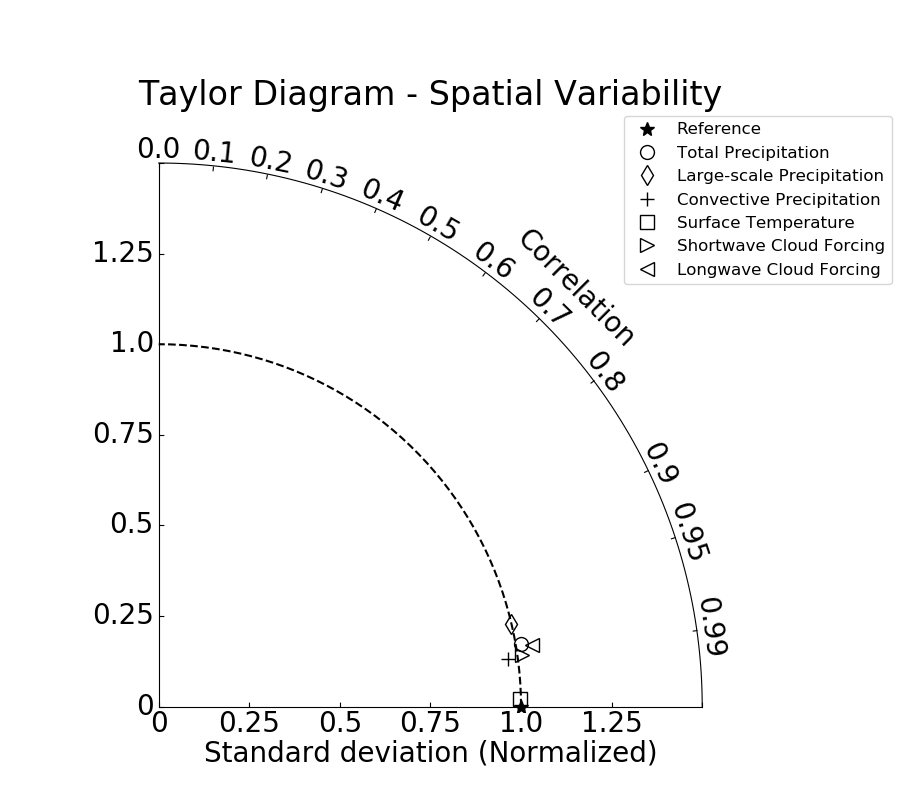
\includegraphics[width=6.5in]{./ANN_metrics_taylor_diag.png}
  \caption{Taylor diagram comparing run with MG2 running at \SI{1}{\second} to run at default settings. Only years \numrange{2}{4} of the simulation were used.}
  \label{e3sm-taylor}
\end{figure}

\begin{figure}[ht]
  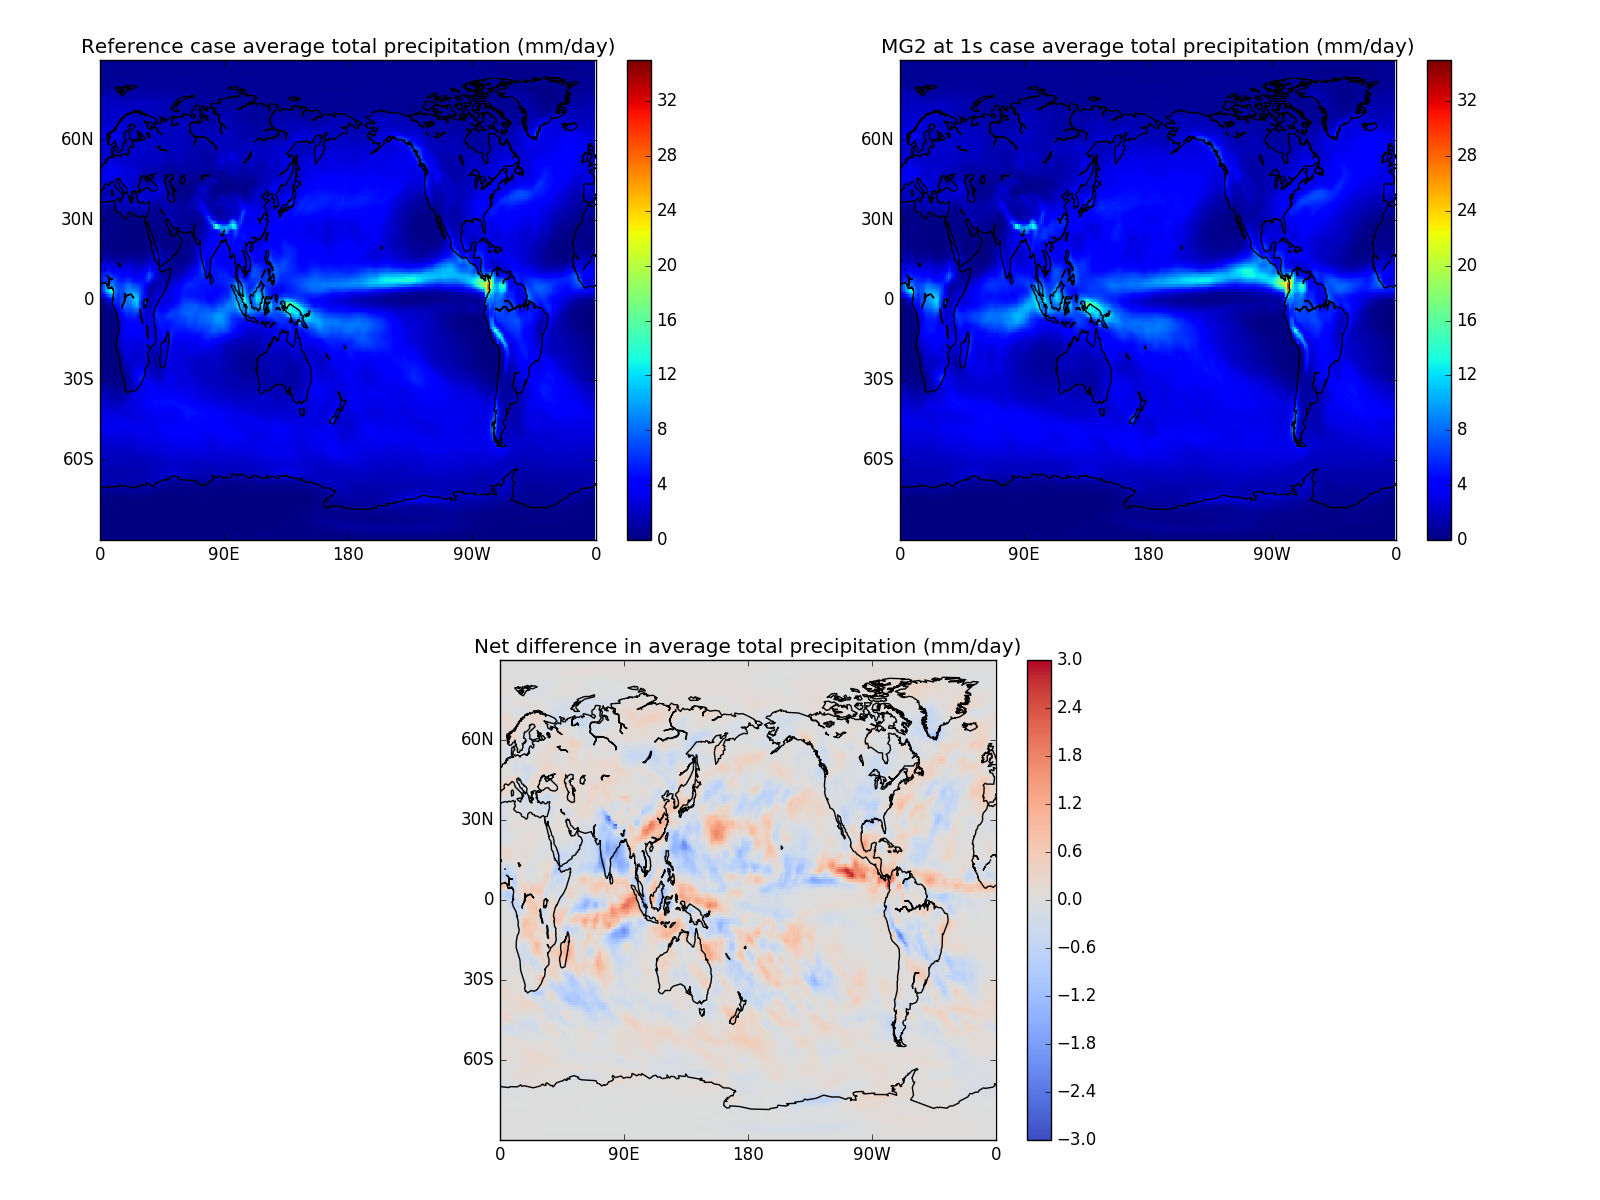
\includegraphics[width=6.5in]{./MG2Figure13.png}
  \caption{Comparison of total precipitation at the surface using MG2 at a \SI{300}{\second} (left) and \SI{1}{\second} (right) time step over three years, with the difference also plotted (center).}
  \label{e3sm-prect-comparison}
\end{figure}

\begin{figure}[ht]
  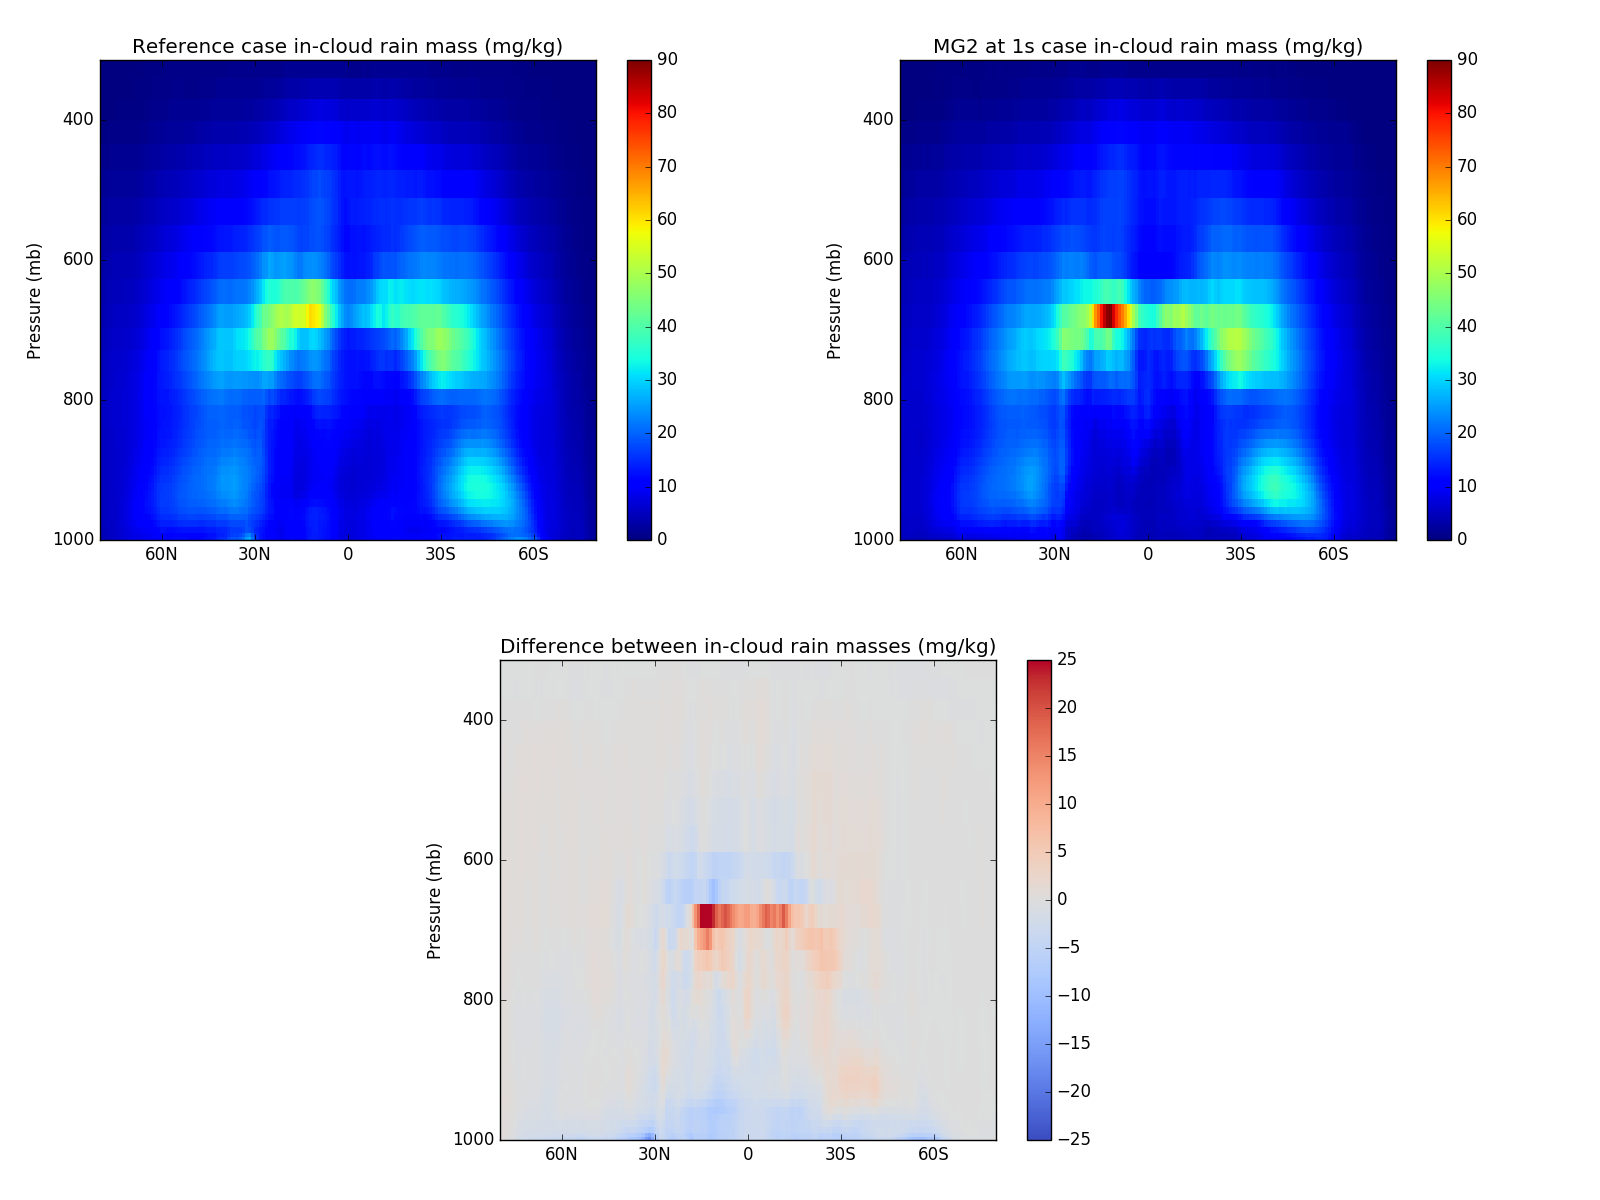
\includegraphics[width=6.5in]{./MG2Figure14.png}
  \caption{Comparison of zonally-averaged rain mass in E3SM runs using MG2 at \SI{300}{\second} (left) and \SI{1}{\second} (right) time step over three years, with the difference also plotted (center).}
  \label{e3sm-rain-comparison}
\end{figure}

\chapter{The Energy Exascale Earth System Model}

\section{Methodology}

We ran E3SM at a $\sim$\SI{100}{\kilo\meter} atmospheric resolution (ne30\_ne30 grid) with standard E3SMv1 tuning and prescribed sea surface temperature. These runs were performed using a maintenance version of E3SM 1.1 (hash 25c94366) with pre-industrial forcings (compset F1850C5AV1C-04P2) unless otherwise specified, and all had prescribed sea surface temperature (SST) and sea ice extent.

The control run (CTRL) is an out-of-the-box run using default settings. We compare this to a new run (ALL10) that changed the atmosphere's dynamics-physics-surface coupling time step, known as ``dtime'' in the model settings, to \SI{10}{\second}. This time step is chosen to be as small as we could reasonably afford, within the constraints of the computing power we had available for this study. CTRL and ALL10 simulations are both \num{3} years in length. Results based on years \numrange{1}{2} were unchanged after adding year \num{3}, which gives us confidence that \num{3} years is long enough to draw robust conclusions.

The dtime setting is often thought of as specifying the entire atmosphere's time step, but there are three ways in which this is not quite true. First, the radiation parameterization uses a fixed time step of once per hour, regardless of dtime. While the ALL10 run does not modify the radiation time step, our tests with shorter runs show that the model is not especially sensitive to this time step. Second, the dynamics and cloud physics contain some substepping by default, though none run at a time step as small as \SI{10}{\second}. In the ALL10 run, we disable these forms of substepping, so that all major dynamics and physics processes aside from radiation run at the same small time step. Third, because the dtime setting also governs the rate at which EAMv1 exchanges information with the surface components, changing it forces a change in the land and sea ice components, which must run at a \SI{10}{\second} time step as well.

To investigate which processes within EAMv1 were most responsible for its overall time step sensitivity, we configured a series of runs using built-in options to substep individual parameterizations at a \SI{10}{\second} time step. These runs include DYN10, which substepped EAMv1's spectral element dynamical core, CLUBB10, which substepped the CLUBB cloud physics parameterization, and MICRO10, which substepped the MG2 stratiform microphysics. Typically CLUBB and MG2 are substepped together within a single loop, so we also produced a CLUBBMICRO10 run that used this capability to run both schemes at \SI{10}{\second}. Because this run showed clear differences from the control, we produced a CLUBBMICRO60 run where CLUBB and MG2 were substepped together at \SI{60}{\second}. Separately, we also produced a CLUBB10MICRO10 run, where the individual time steps for CLUBB and MG2 were reduced, but the two schemes were only coupled at the default rate of once per \SI{300}{\second}. To verify our prior belief that the model is less sensitive to the radiation time step size than to other physics time steps, we produced the ALLRAD10 run, which is identical to the ALL10 run except that the radiation is also run at a \SI{10}{\second} time step. Finally, we produced the ALL300 and ALL60 runs, which change dtime to \SI{300}{\second} and \SI{60}{\second}, respectively. ALL300 is useful as an additional control, because it decreases the dynamics-physics coupling time step, but does not decrease the CLUBB or MG2 time steps, nor does it decrease the dynamics time steps (except the remapping for the vertically Lagrangian advection scheme, which normally runs every \SI{900}{\second}). A summary of all these runs can be found in Table \ref{tab:runs}.

\begin{table}
  \centering
  \footnotesize
  \begin{tabular}{|c|p{0.4\linewidth}|r|r|}
    \hline
    Name & Substepped processes & Substep size & Run length \\
    \hline
    CTRL & None & N/A & \SI{38}{\month} \\
    \hline
    ALL10 & Dynamics-physics coupling & \SI{10}{\second} & \SI{38}{\month} \\
    ALL60 & & \SI{60}{\second} & \SI{30}{d} \\
    ALL300 & & \SI{300}{\second} & \SI{30}{\day} \\
    \hline
    DYN10 & Dynamics and tracer advection & \SI{10}{\second} & \SI{30}{\day} \\
    \hline
    MICRO10 & MG2 microphysics & \SI{10}{\second} & \SI{30}{\day} \\
    \hline
    CLUBB10 & CLUBB unified cloud parameterization & \SI{10}{\second} & \SI{30}{\day} \\
    \hline
    CLUBB10MICRO10 & CLUBB and MG2 & \SI{10}{\second} & \SI{30}{\day} \\
    \hline
    CLUBBMICRO10 & CLUBB+MG2 combined loop & \SI{10}{\second} & \SI{30}{\day} \\
    CLUBBMICRO60 & & \SI{60}{\second} & \\
    \hline
    ALLRAD10 & Dynamics-physics coupling and radiation & \SI{10}{\second} & \SI{30}{\day} \\
    \hline
  \end{tabular}
  \caption{Runs performed using the default aerosol scheme.}
  \label{tab:runs}
\end{table}

In EAMv1, the most important parameterization that does \emph{not} have this built-in substepping capability is the ZM deep convection, which always runs at the time step given by dtime. Substepping this parameterization individually is challenging and is described further in section \ref{sec:zm-substep}.

\section{Results}

\subsection{Effects of Decreasing the Physics Time Step}

Consistent with the literature on CAM, we find a \SI{0.08}{\milli\meter\per\day} increase in global-mean total precipitation with \SI{10}{\second} time steps, mostly stemming from low latitudes. While convective precipitation decreases, large-scale precipitation increases by $\sim$\SI{60}{\percent} in the tropics (defined here as latitudes from \num{30}S to \num{30}N), especially over land (Figure \ref{fig:all10-prec-map}a). The overall effect is an increase in tropical precipitation over the Pacific warm pool, and a near-doubling of precipitation in parts of Borneo, New Guinea, and Colombia (Figure \ref{fig:all10-prec-map}b).

\begin{figure}
    \centering
    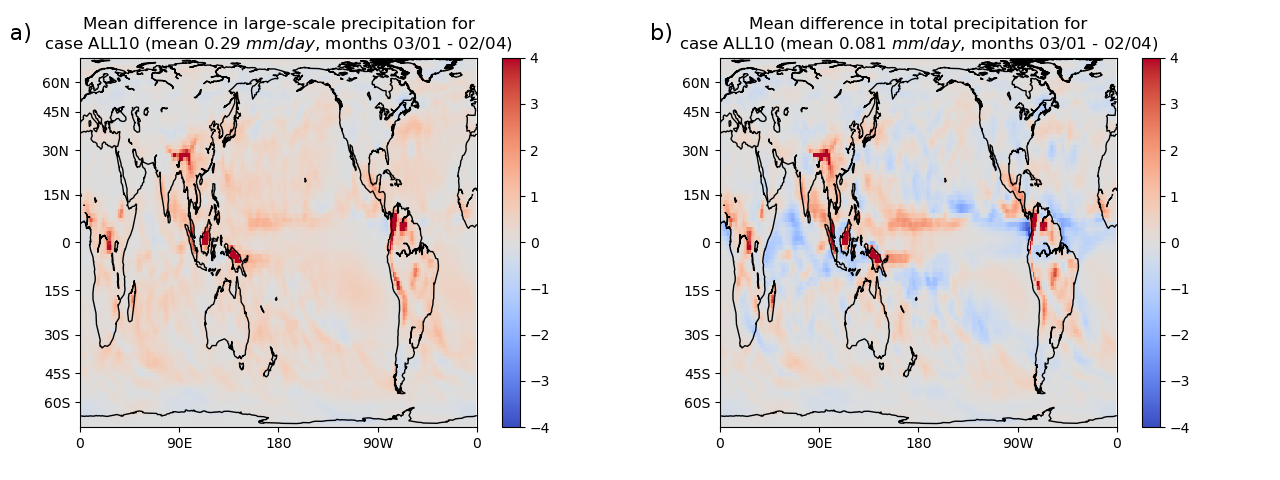
\includegraphics[width=5.5in]{Figure1.png}
    \caption{Differences in a) large-scale precipitation and b) total precipitation between CTRL and ALL10 runs.}
    \label{fig:all10-prec-map}
\end{figure}

Evaporation must increase to fuel the precipitation increases.  Over the oceans, this is due to slightly higher wind speed and lower near-surface relative humidity. The average \SI{10}{\meter} wind speed in the tropics increases from \SIrange{5.56}{5.70}{\meter\per\second}, and occurs mainly in the northern Indian ocean and central Pacific, while latent heat flux increases in the same areas, by about \SI{4}{\watt\per\meter\squared} (not shown). This is consistent with the CAM3 literature, suggesting that an increase in wind speed contributes an increase in evaporation for short time steps.

Unlike in CAM3, the relative humidity decreases throughout the troposphere in the ALL10 run, as shown in Figure \ref{fig:all10-relhum-map}. The decreases in the \SIrange[range-phrase=--,range-units=single]{800}{850}{\millibar} layer correspond to a significant reduction in low cloud mass (Figure \ref{fig:all10-wp-map}). This suggests that the increase in precipitation is caused primarily by increased precipitation efficiency. At the same time, we see an increase in cloud liquid above the boundary layer, particularly at high latitudes. In the ALL10 run, the cloud fraction not only decreases at lower levels, where less liquid cloud is present, but also at higher levels, where the average cloud mass mixing ratios are similar to or greater than their values in CTRL (Figure \ref{fig:all10-cld-map}).

\begin{figure}
    \centering
    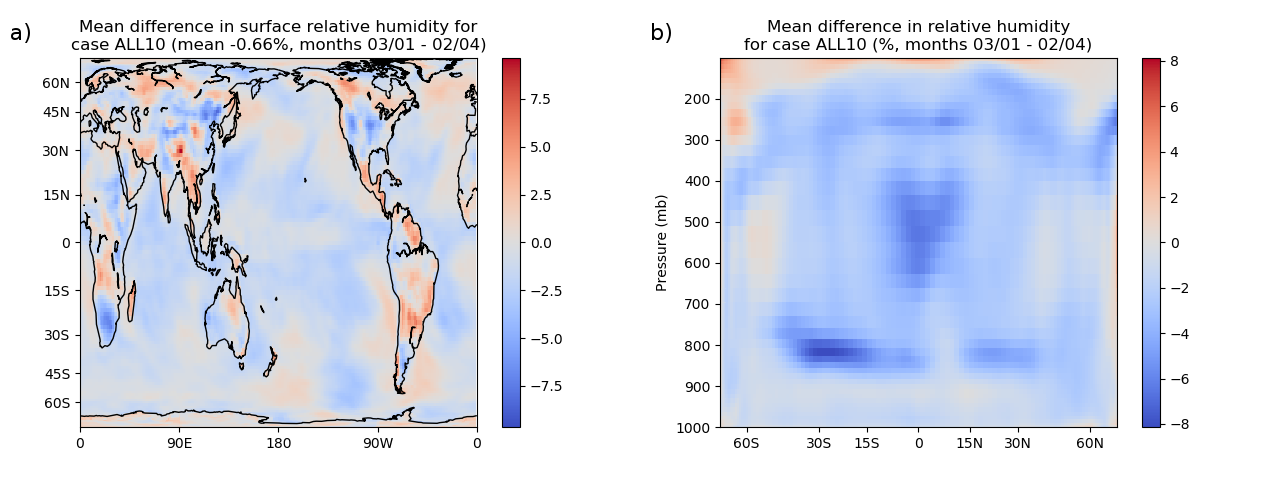
\includegraphics[width=5.5in]{Figure2.png}
    \caption{Differences in a) relative humidity and b) zonal mean relative humidity between CTRL and ALL10 runs.}
    \label{fig:all10-relhum-map}
\end{figure}

\begin{figure}
    \centering
    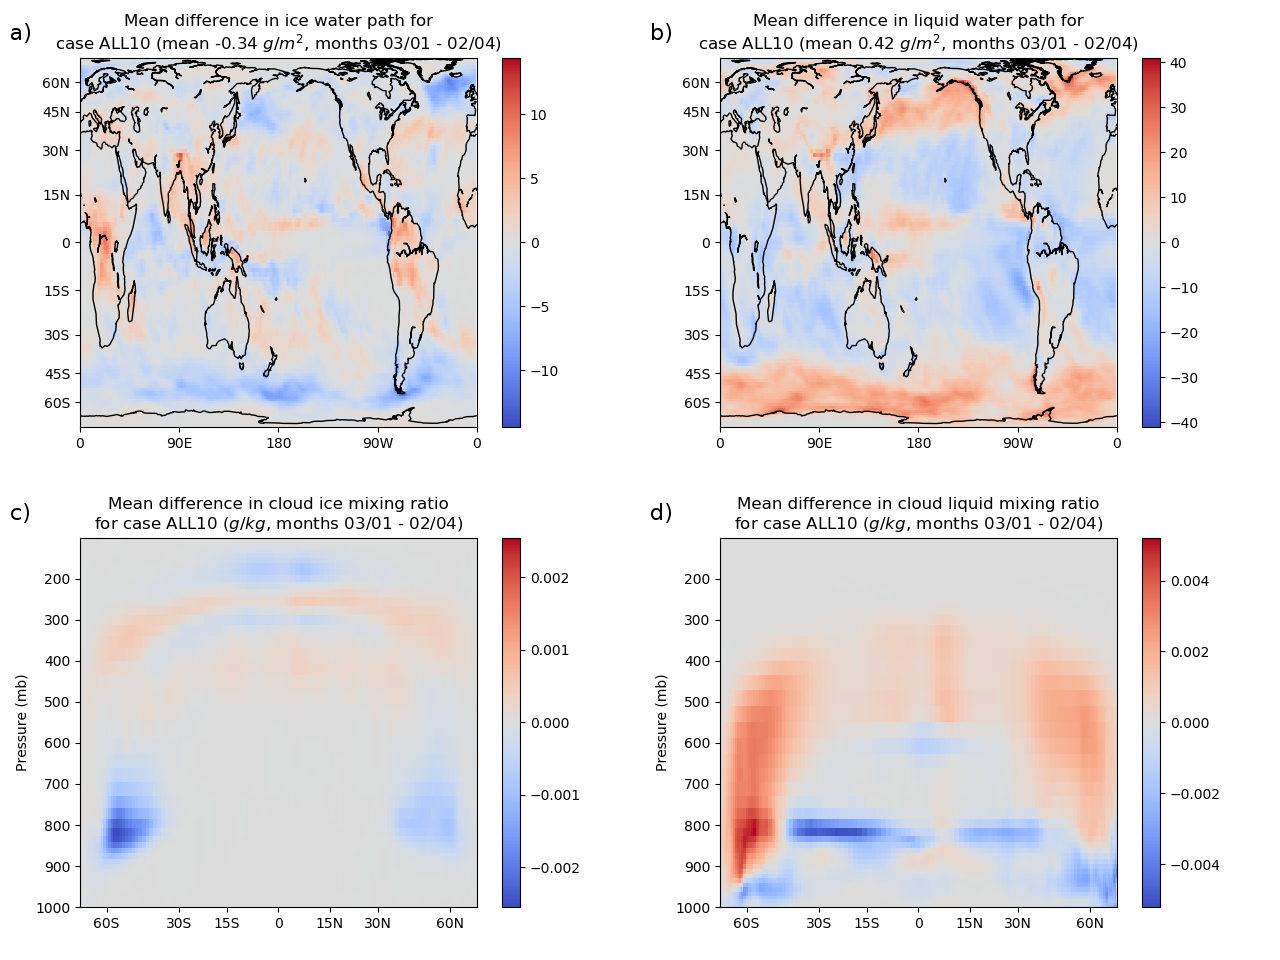
\includegraphics[width=5.5in]{Figure3.png}
    \caption{Differences in mass of cloud ice and liquid water between CTRL and ALL10 runs, measured by a) ice water path, b) liquid water path, c) zonal mean cloud ice mixing ratio, and d) zonal mean cloud liquid mixing ratio.}
    \label{fig:all10-wp-map}
\end{figure}

\begin{figure}
    \centering
    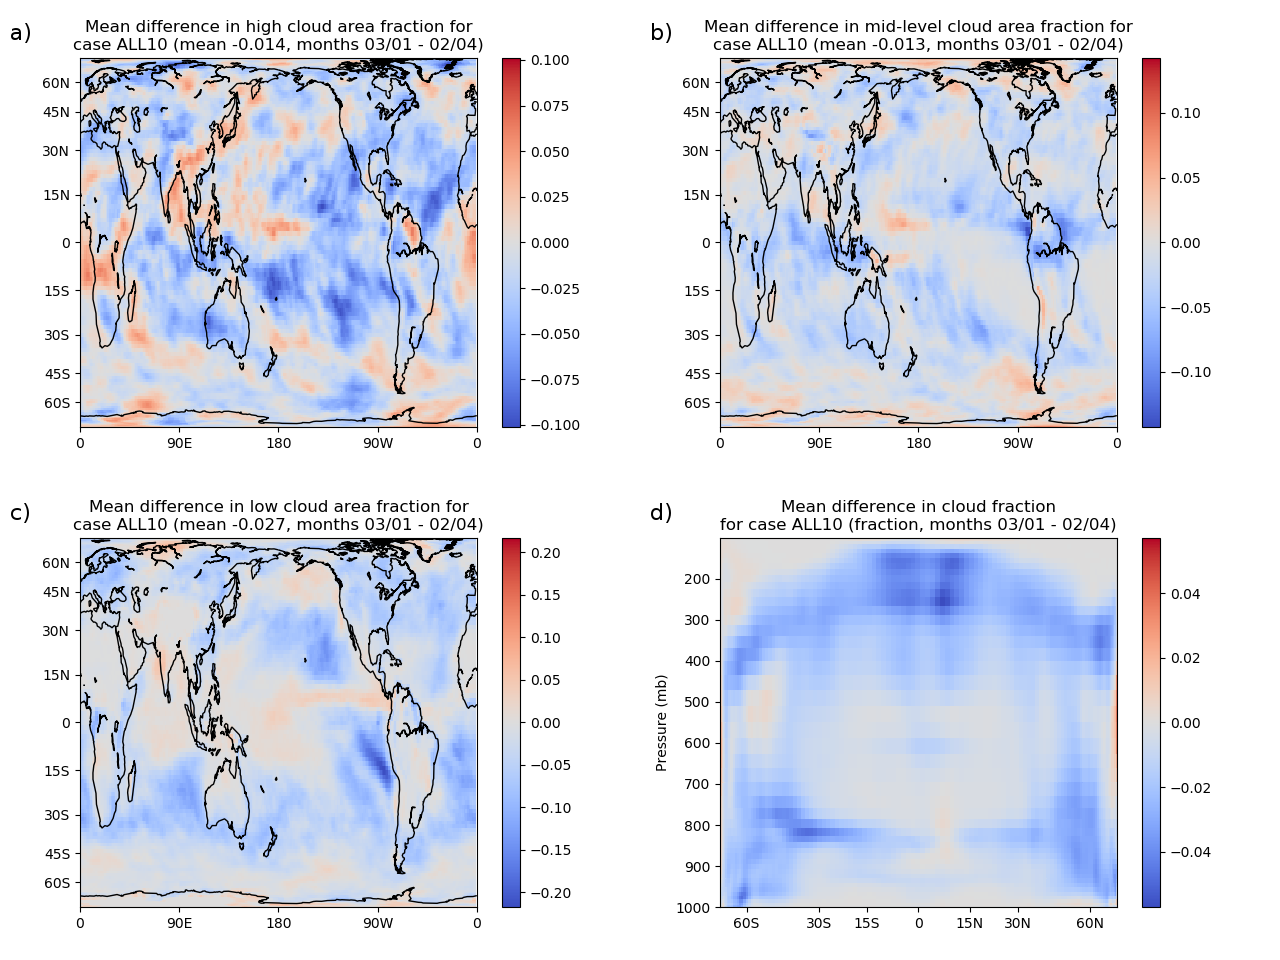
\includegraphics[width=5.5in]{Figure4.png}
    \caption{Differences in cloud fraction between CTRL and ALL10 runs: a) high cloud fraction (defined as the vertical integral above \SI{400}{\millibar}), b) mid-level cloud fraction (vertical integral over the range \SIrange[range-phrase=--,range-units=single]{400}{700}{\millibar}), c) low cloud fraction (vertical integral below \SI{700}{\millibar}), and d) zonal mean cloud fraction at each level.}
    \label{fig:all10-cld-map}
\end{figure}

Consistent with the decrease in overall cloud mass and fraction, the ALL10 run shows substantially reduced radiative cloud forcing compared with CTRL, as can be seen in Figure \ref{fig:all10-cf-map}. The effect on shortwave cloud forcing is especially large, the global mean being reduced from \SI{-43.0}{\watt\per\meter\squared} to \SI{-37.5}{\watt\per\meter\squared}.

\begin{figure}
    \centering
    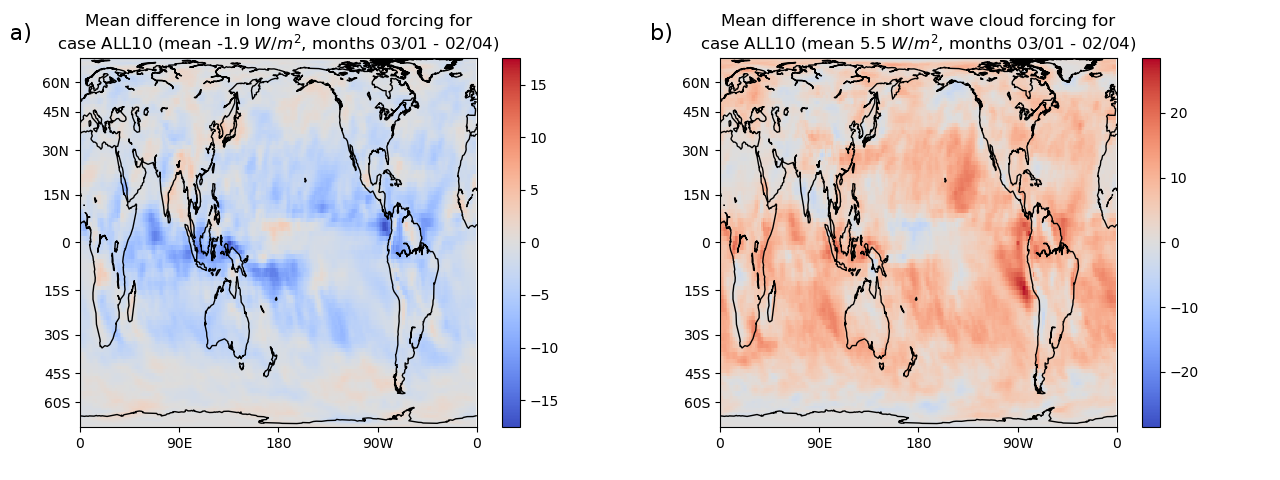
\includegraphics[width=5.5in]{Figure5.png}
    \caption{Differences in a) longwave cloud forcing and b) shortwave cloud forcing between CTRL and ALL10 runs.}
    \label{fig:all10-cf-map}
\end{figure}

Spatial-pattern differences between CTRL and ALL10 are summarized by a Taylor diagram shown in Figure \ref{fig:taylor}. We find that the effect of reducing the model time step to \SI{10}{\second} (black symbols) is comparable to the effect of doubling the model's horizontal grid spacing (red symbols), a natural standard for comparison. Historically, spatial resolution changes have been perceived as a major model change while accompanying time step changes have been taken for granted; Figure \ref{fig:taylor} illustrates that this viewpoint has shortcomings. The variables most affected by the time step are related to precipitation, with the large-scale precipitation showing the most difference.

\begin{figure}
    \centering
    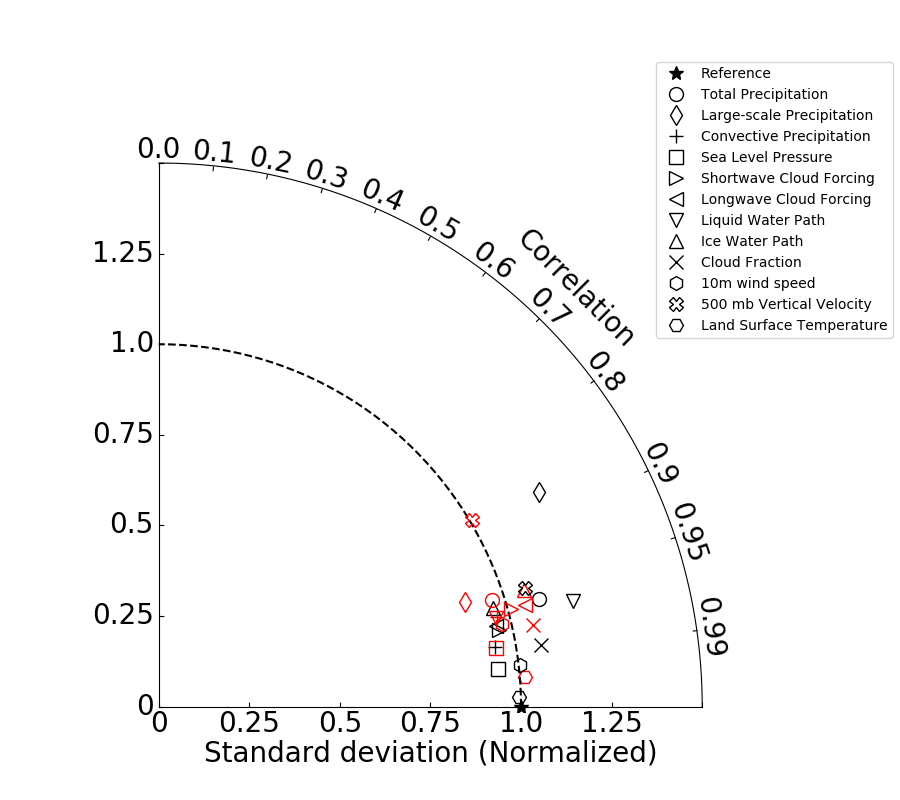
\includegraphics[width=5.5in]{Figure6.png}
    \caption{Taylor diagram comparing results from the CTRL and ALL10 runs (black), and comparing results from CTRL to a run with default settings using the ne16 grid (red), which has a grid spacing of $\sim$\ang{1.9}. This diagram uses values averaged over a three year time period starting March of the first simulated year for each run; only spatial variability is accounted for.}
    \label{fig:taylor}
\end{figure}

\subsection{Effects of Changing the Physics Substepping}

We did not have the computational resources to run all of our substepped configurations for multiple years, but many of the effects of substepping are quite large and can easily be distinguished with only a few days of data. Since all runs started with the same initial conditions, they followed a similar trajectory for the first \num{15} days before beginning to diverge, so we focused on comparing the runs during this time period. (In Figure \ref{fig:cld-frc}, we have included data from \num{30} days, which shows an example of how, in these different runs, the global means of cloud-related variables become significantly less correlated towards the end of the month.)

We first examine the changes in precipitation across these runs, shown in Figure \ref{fig:precl-prect}. We can categorize our runs into five main categories based on large-scale precipitation:

\begin{enumerate}
\item The lowest average large-scale precipitation rates are found in CTRL, CLUBB10, and DYN10, suggesting that the cloud physics is not sensitive to the CLUBB or dynamics time steps.
\item A slightly higher large-scale precipitation rate is found in the ALL300 run, which has a reduced time step for the ZM deep convection and an increased dynamics-physics coupling frequency, but does not change the CLUBB or MG2 time steps. This run shows a mild repartitioning of precipitation from the convective to large-scale category, perhaps consistent with the mechanisms described in \cite{Williamson2013}.
\item The MICRO10 and CLUBB10MICRO10 runs show signs of increased precipitation efficiency overall, increasing both large-scale \emph{and} total precipitation.
\item One of the largest large-scale precipitation rates comes from CLUBBMICRO10, which couples CLUBB to MG2 every \SI{10}{\second}, suggesting that an increase in CLUBB-MG2 coupling frequency has an additional effect beyond that from simply substepping MG2 more frequently. CLUBBMICRO60 may see a similar effect, though it is not as clearly distinguished from the MICRO10 run.
\item The ALL10 and ALLRAD10 runs decrease both the dynamics-physics coupling time step and the time step used for all physics parameterizations, and these show the largest changes in precipitation.
\end{enumerate}

\begin{figure}
    \centering
    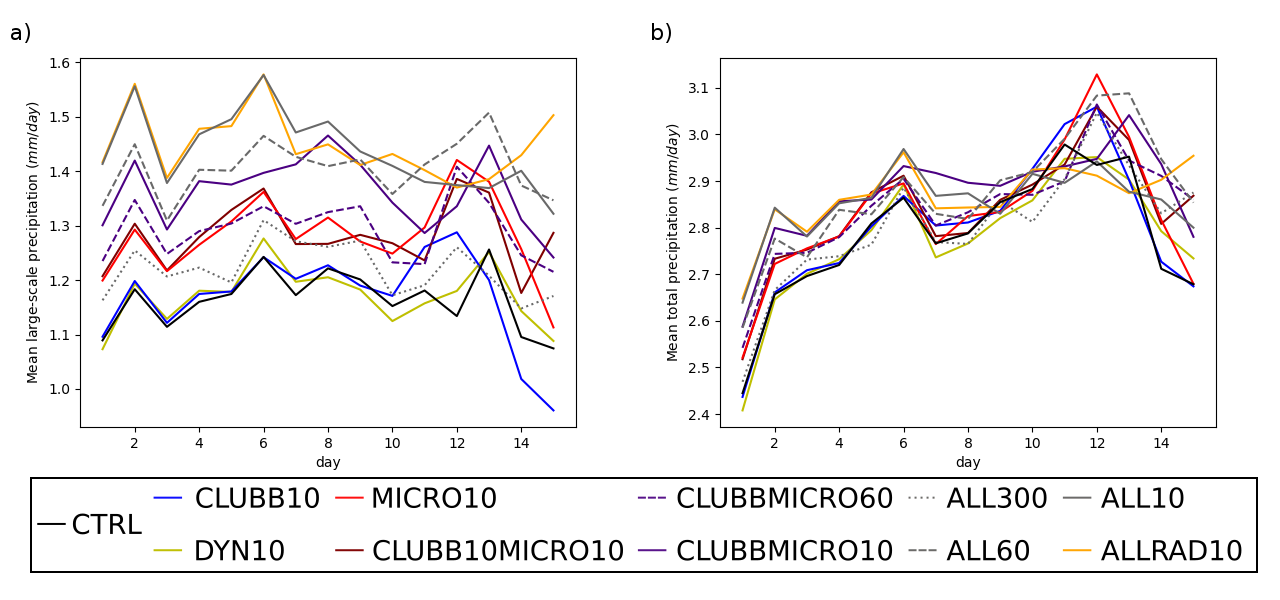
\includegraphics[width=5.5in]{Figure7.png}
    \caption{Daily global means of a) large-scale precipitation only and b) total precipitation for substepped runs.}
    \label{fig:precl-prect}
\end{figure}

While the increase in large-scale precipitation seen in the MICRO10 run is substantial, the spatial pattern is quite different from the ALL10 case, as seen in Figure \ref{fig:precl-map}. In particular, the patterns observed in the ALL10 case, such as the increase in large-scale precipitation over land, only appear when both CLUBB and MG2 are substepped together, as in the CLUBBMICRO10 case. We have also plotted the CLUBB10MICRO10 case, to show that this difference is not due simply to the reduction in the CLUBB time step alone.

\begin{figure}
    \centering
    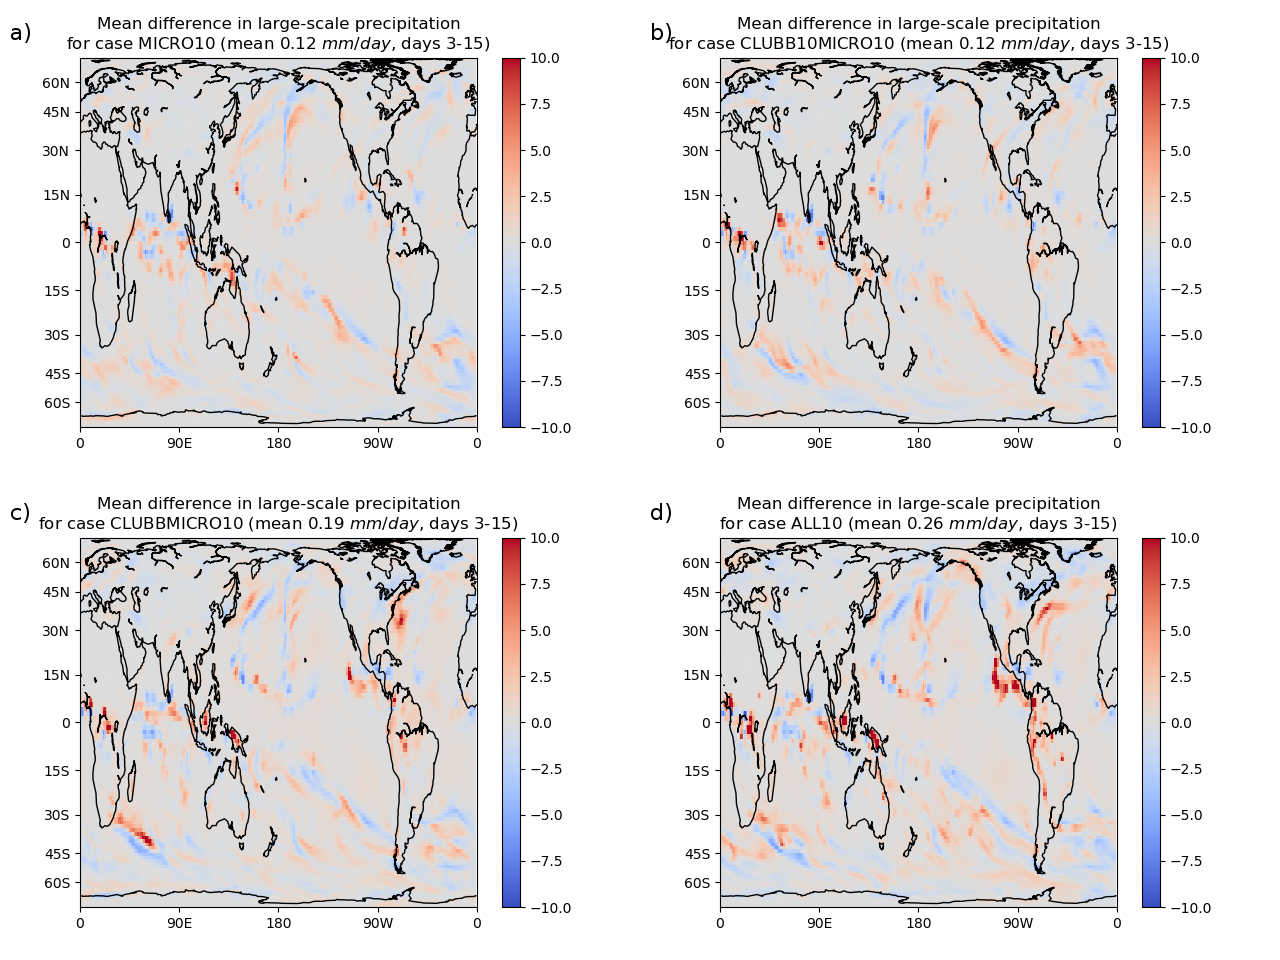
\includegraphics[width=5.5in]{Figure8.png}
    \caption{Differences in large-scale precipitation versus CTRL for a) MICRO10, b) CLUBB10MICRO10, c) CLUBBMICRO10, and d) ALL10.}
    \label{fig:precl-map}
\end{figure}

Together, these results suggest that the main time steps affecting the precipitation are the MG2 microphysics time step and the coupling time step between the CLUBB and MG2 schemes. The change in the CLUBB and MG2 combined time step therefore explains most of the precipitation change noted earlier between the CTRL and ALL10 runs. Either the dynamics-physics coupling time step or the ZM deep convection time step could also be affecting the precipitation between the convective and large-scale processes, since both these time steps are changed in the ALL10 and ALL300 runs. We will investigate this further in Section \ref{sec:zm-substep}. The changes in total precipitation are mostly apparent for the first week of the run, after which the runs with default MG2 time step see a significant increase in convective precipitation (not shown), leading to no systematic difference between simulations after this point.

The particular pattern of decreased relative humidity found in the ALL10 run also appears in the CLUBBMICRO10 run, but not the MICRO10 run (not shown). However, as shown in Figure \ref{fig:cldliq-map}, the cloud liquid in the CLUBBMICRO10 run only matches the ALL10 run at low altitudes, while the ALL300 run is much more effective at matching ALL10 at higher altitudes, suggesting that the dynamics-physics coupling time step is responsible for these increases in cloud liquid. The CLUBBMICRO10 also consistently produces clouds in the lowest level of the atmosphere over land, particularly in South America and Southeast Asia, which are not seen in any other run. This may be an artifact resulting from CLUBB and MG2 running at a time step much smaller than the atmosphere-land coupling interval.

\begin{figure}
    \centering
    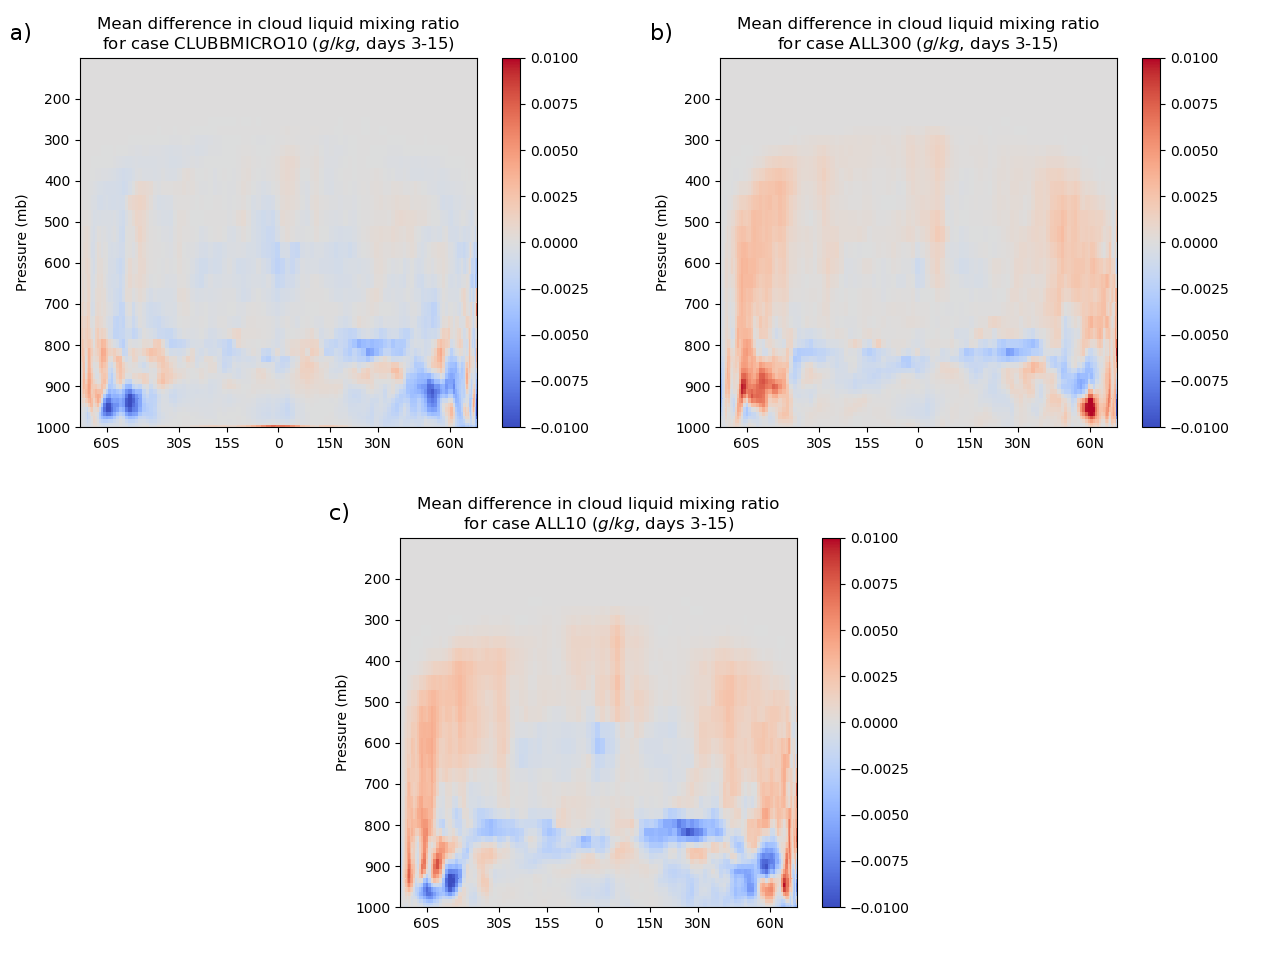
\includegraphics[width=5.5in]{Figure9.png}
    \caption{Differences in zonal mean cloud liquid mixing ratio versus CTRL for a) ALL300, b) CLUBBMICRO10, and c) ALL10.}
    \label{fig:cldliq-map}
\end{figure}

The overall differences in ice and liquid water path are shown in Figure \ref{fig:water-path}. We see that, in the tropics, the runs with reduced MG2 time step reduce the liquid water path in a way that is similar to the ALL10 run, while the ALL300 run increases the ice and liquid water path everywhere. We also note that if MG2 is substepped independently from CLUBB, the ice water path increases significantly, but this does not occur when MG2 and CLUBB are substepped together.

\begin{figure}
    \centering
    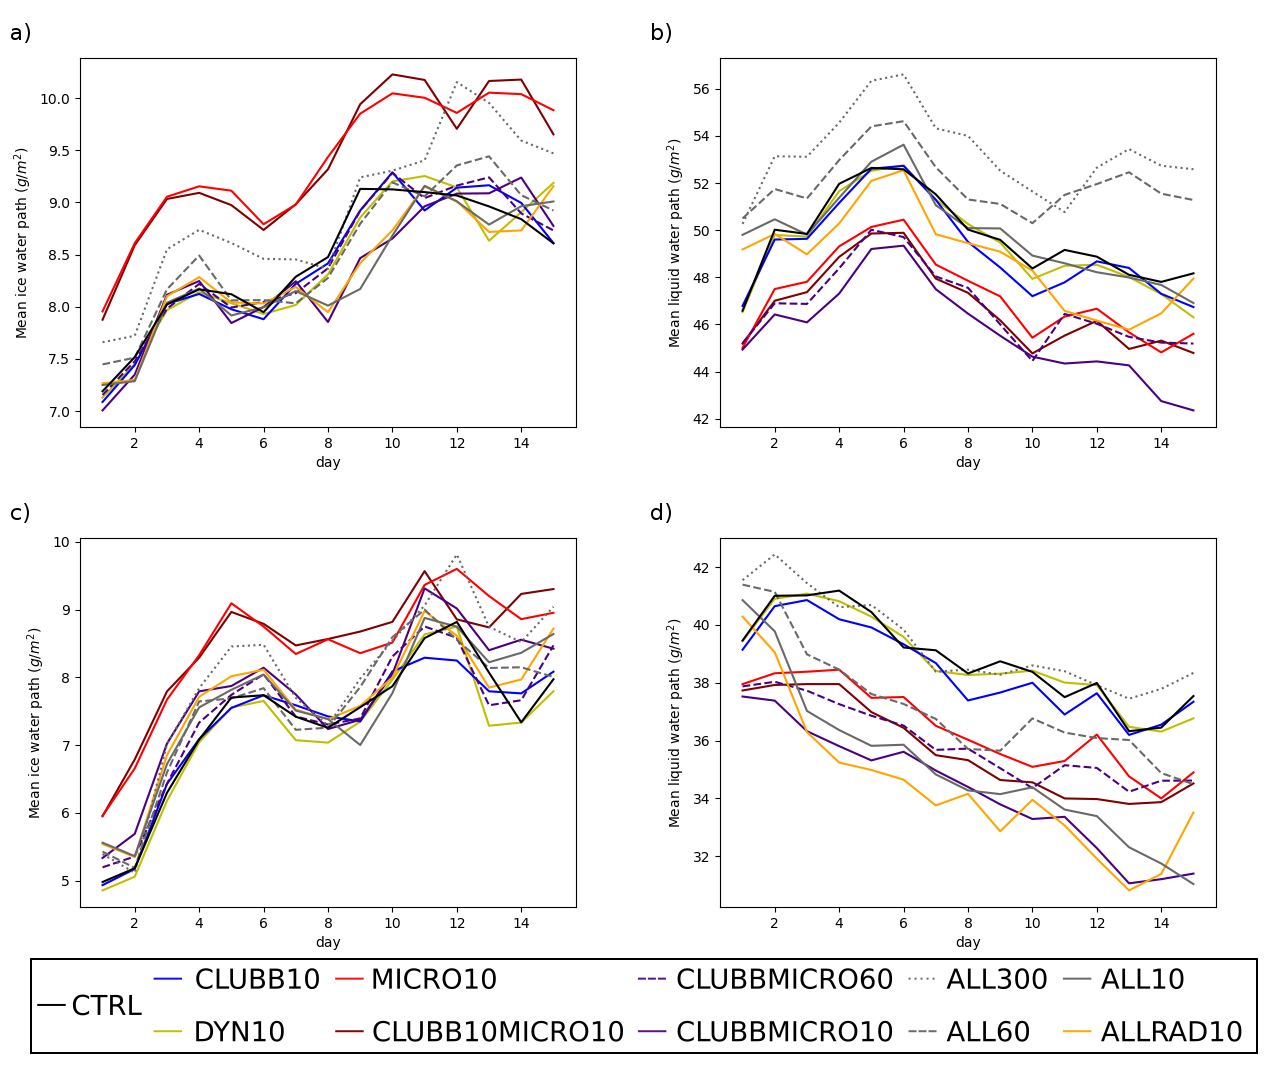
\includegraphics[width=5.5in]{Figure10.png}
    \caption{Daily means for a,c) ice water path and b,d) liquid water path for substepped runs. Plots a-b) show global means, while c-d) show means over low latitude grid points (\num{30}S--\num{30}N).}
    \label{fig:water-path}
\end{figure}

We noted earlier that the ALL10 run caused a reduction in cloud fraction throughout most of the atmosphere, especially in the low cloud fraction. As shown in Figure \ref{fig:cldlow-cldmed}, this effect seems to have different causes, depending on which level of the atmosphere is examined. Reductions in low cloud are primarily due to the reduction in the dynamics-physics coupling substep, but the CLUBB and MG2 combined time step has a greater effect on the cloud fraction above \SI{700}{\millibar}.

\begin{figure}
    \centering
    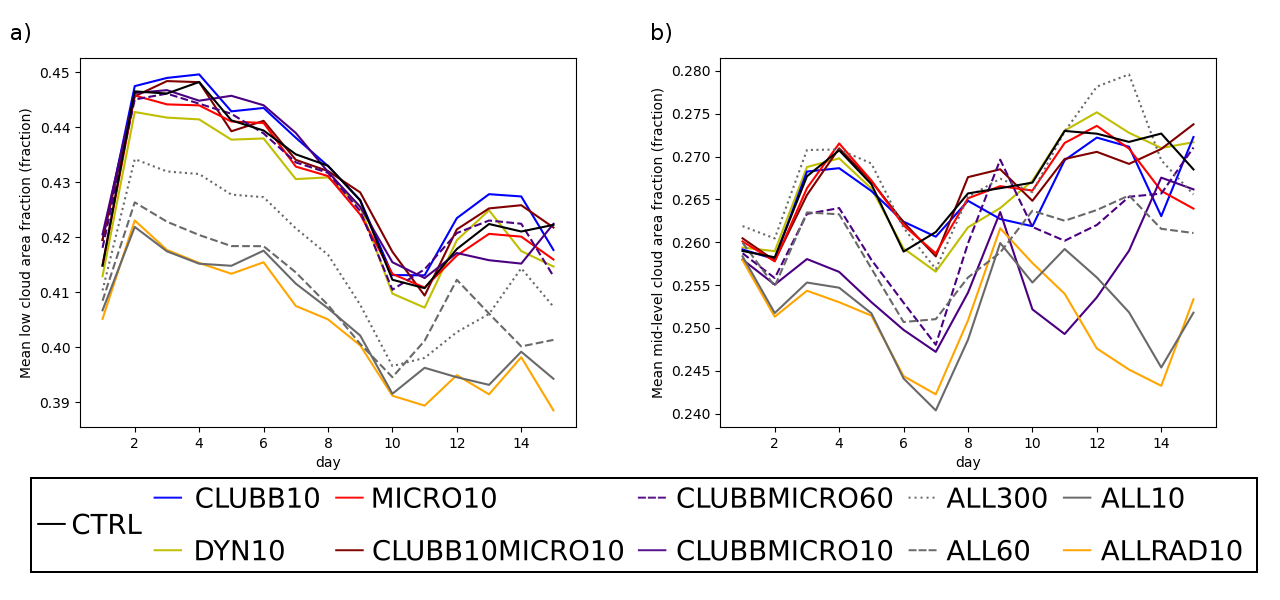
\includegraphics[width=5.5in]{Figure11.png}
    \caption{Daily global means of a) low cloud fraction ($>$ \SI{700}{\millibar}), and b) mid-level cloud fraction (\SIrange[range-phrase=--,range-units=single]{400}{700}{\millibar}) for substepped runs.}
    \label{fig:cldlow-cldmed}
\end{figure}

Finally, we turn to the changes in radiative cloud forcing between runs. The magnitudes of both shortwave and longwave cloud forcing are reduced in the ALL10, ALLRAD10, CLUBBMICRO10, and CLUBBMICRO60 runs, likely due to the significant decreases in cloud fraction and liquid water path found in the tropics. The MICRO10 and CLUBB10MICRO10 runs, on the other hand, have a much larger ice water path, leading to an increase in longwave cloud forcing. The ALL300 run has both a reduced low cloud fraction and an increase in liquid and ice water path, leading to a decrease in shortwave cloud forcing and no net change in longwave cloud forcing.

\begin{figure}
    \centering
    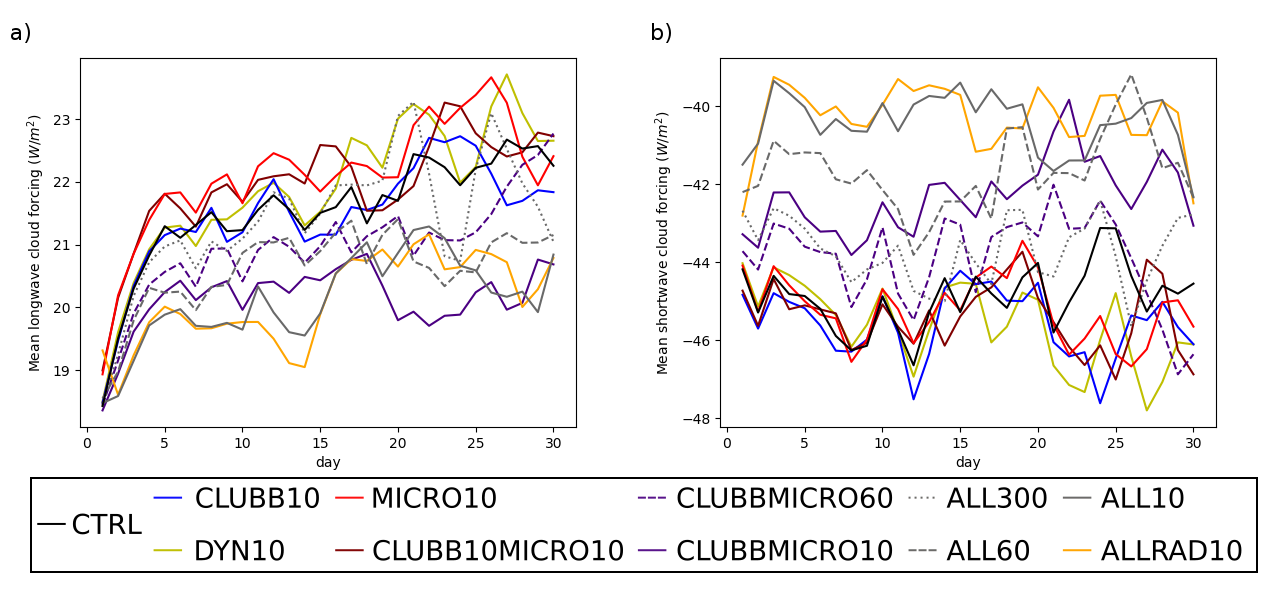
\includegraphics[width=5.5in]{Figure12.png}
    \caption{Daily global means of a) longwave cloud forcing and b) shortwave cloud forcing for substepped runs.}
    \label{fig:cld-frc}
\end{figure}

We notice that most variables take a few days for the differences between runs to fully develop, but the effect of a change in the MG2 time step strongly affects large-scale precipitation and ice water path within the first day. We suspect that most effects of a decreased time step require a certain degree of "spin up" in order for runs starting with the same initial condition to become more distinct. We hypothesize that the more instantaneous changes are primarily due to the direct effects of a decreased time step on microphysical process rates, which can respond directly and dramatically to changes in time step \parencite{Santos2020}.

\subsection{Substepping the ZM Deep Convection Scheme}

\label{sec:zm-substep}

So far, we have been unable to distinguish between the effect of substepping the ZM deep convection scheme and the effect of reducing the dynamics-physics coupling time step. In order to explore the effect of ZM substepping on results, we produced a simple set of code modifications to EAMv1 to allow this scheme to be substepped on its own. Most of these modifications are straightforward, since the main effect of ZM is simply to modify the state of the atmosphere for the next parameterization in the sequentially split physics. Two of ZM's outputs are precipitation process rates that are used by the modal aerosol scheme to calculate the total precipitation produced/evaporated by the deep convection. These rates are averaged over the whole time step in our modifications.

With this modified version of EAMv1, we were able to run the deep convection at a somewhat lower time step size, down to \SI{300}{\second}. However, the model becomes unstable if the ZM deep convection is a smaller time step (\SI{60}{\second} or less) while the rest of the model runs at a default time step. Specifically, the wet deposition routines in the modal aerosols behave inappropriately, causing an unphysical increase in aerosol mass due to excessive water uptake, which in turn causes the aerosol optical depth to increase exponentially until the model crashes. Even in runs that did not crash, this behavior was present and had a significant impact on model physics. We were therefore unable to investigate the effect of ZM substepping further using the model's default configuration.

Fortunately, we do have an alternative, which is to run the model with prescribed aerosols, an ability commonly used for single column runs \parencite{LebassiHabtezion2015}. This required switching to a configuration where prescribed aerosol data was available, so we used a year \num{2000} compset, FC5AV1C-04P2. As a result, these results cannot be directly compared to our previous runs, though we used the same spatial grid, and the physics of this compset is similar to our previous runs, aside from initial/boundary conditions. We reproduced the CTRL, ALL10, and CLUBBMICRO10 runs using prescribed aerosols, and further produced runs that substep ZM by itself, as well as runs that substep ZM and CLUBB/MG2 separately, and finally a run that substeps all three parameterizations. These simulations are summarized in Table \ref{tab:pa-runs}.

\begin{table}
  \centering
  \begin{tabular}{|c|p{0.3\linewidth}|r|r|}
    \hline
    Name & Substepped processes & Substep size & Run length \\
    \hline
    CTRLPA & None & N/A & \SI{30}{\day} \\
    \hline
    ALL10PA & Dynamics-physics coupling & \SI{10}{\second} & \SI{30}{\day} \\
    \hline
    CLUBBMICRO10PA & CLUBB+MG2 combined loop & \SI{10}{\second} & \SI{30}{\day} \\
    \hline
    ZM10PA & ZM deep convection & \SI{10}{\second} & \SI{30}{\day} \\
    \hline
    CLUBBMICRO10ZM10PA & CLUBB+MG2 combined loop and ZM deep convection & \SI{10}{\second} & \SI{30}{\day} \\
    \hline
    CLD10PA & CLUBB+MG2+ZM combined loop & \SI{10}{\second} & \SI{30}{\day} \\
    \hline
  \end{tabular}
  \caption{Runs performed using prescribed aerosols}
  \label{tab:pa-runs}
\end{table}

First, we note that the CLD10PA run, which substeps the ZM deep convection along with CLUBB and MG2 in a single loop, has the same effect on the partitioning of precipitation as seen in the ALL10PA run, being even closer to those results than the CLUBBMICRO10PA run was. This difference can be seen in Figure \ref{fig:precl-prect-pa}, and suggests that the reduced ZM-CLUBB-MG2 coupling time step was responsible for the increased large-scale precipitation seen in the ALL300 and ALL10 runs in Figure \ref{fig:precl-prect}. Figure \ref{fig:precl-prect-pa} also shows that substepping ZM \emph{by itself} has no effect on precipitation, since the ZM10PA run is similar to CTRLPA and the CLUBBMICRO10ZM10PA run is similar to CLUBBMICRO10PA. \cite{Williamson2013} shows that the ZM scheme is not very active when coupled to other parameterizations at small time step sizes, when using a typical value of the convective relaxation time-scale (on the order of \num{1} hour, which is also the value in our experiments). We see the same shift from deep convection towards stratiform precipitation at short time steps.

\begin{figure}
    \centering
    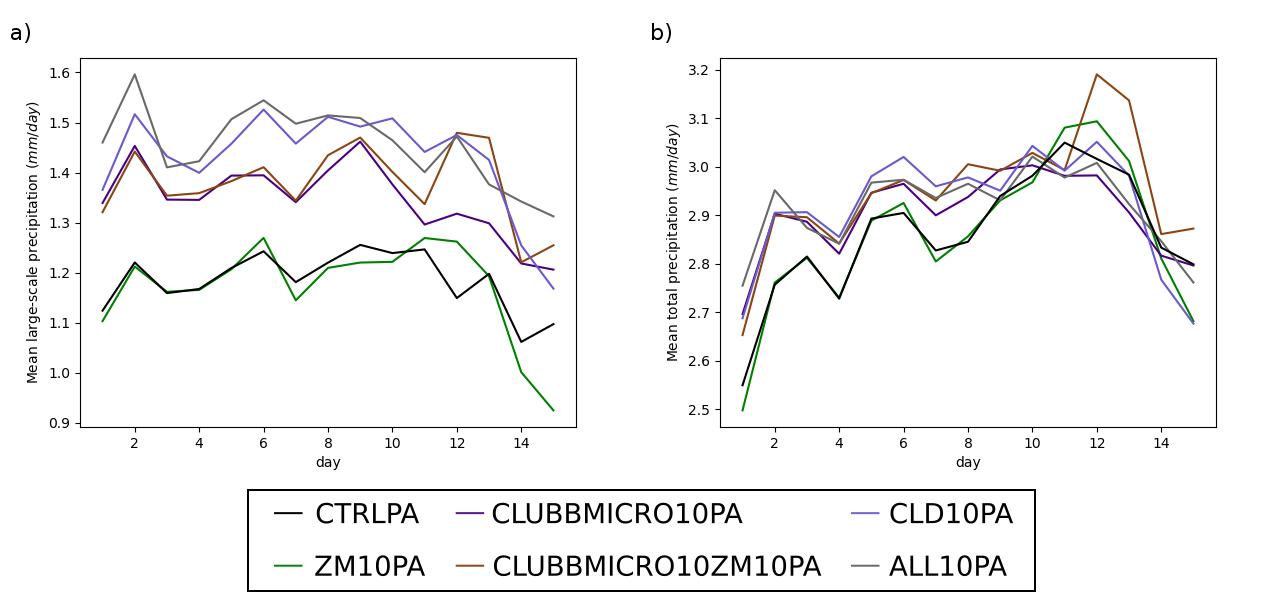
\includegraphics[width=5.5in]{Figure13.png}
    \caption{Daily global means of a) large-scale precipitation only and b) total precipitation for prescribed aerosol substepped runs.}
    \label{fig:precl-prect-pa}
\end{figure}

Second, we note that deep convection substepping, like substepping of the other parameterizations, causes a decrease in low cloud liquid mass, and contributes to the overall pattern seen in the ALL10PA run. This is seen in Figure \ref{fig:cldliq-pa}, where the distribution of liquid water below \SI{750}{\millibar} agrees quite well between the CLD10PA run and the ALL10PA run. However, the increase in cloud liquid above this level is still absent from the CLD10PA run, implying that that increase requires more frequent dynamics-physics coupling to occur. This means that the CLD10PA "overshoots" the ALL10PA run in the tropics, having an even lower liquid water path. Unlike the effect of ZM substepping on precipitation, the effect on cloud liquid does not rely on coupling with CLUBB and MG2, since the CLUBBMICRO10ZM10PA run (not shown) and the CLD10PA run have fairly similar liquid water path.

\begin{figure}
    \centering
    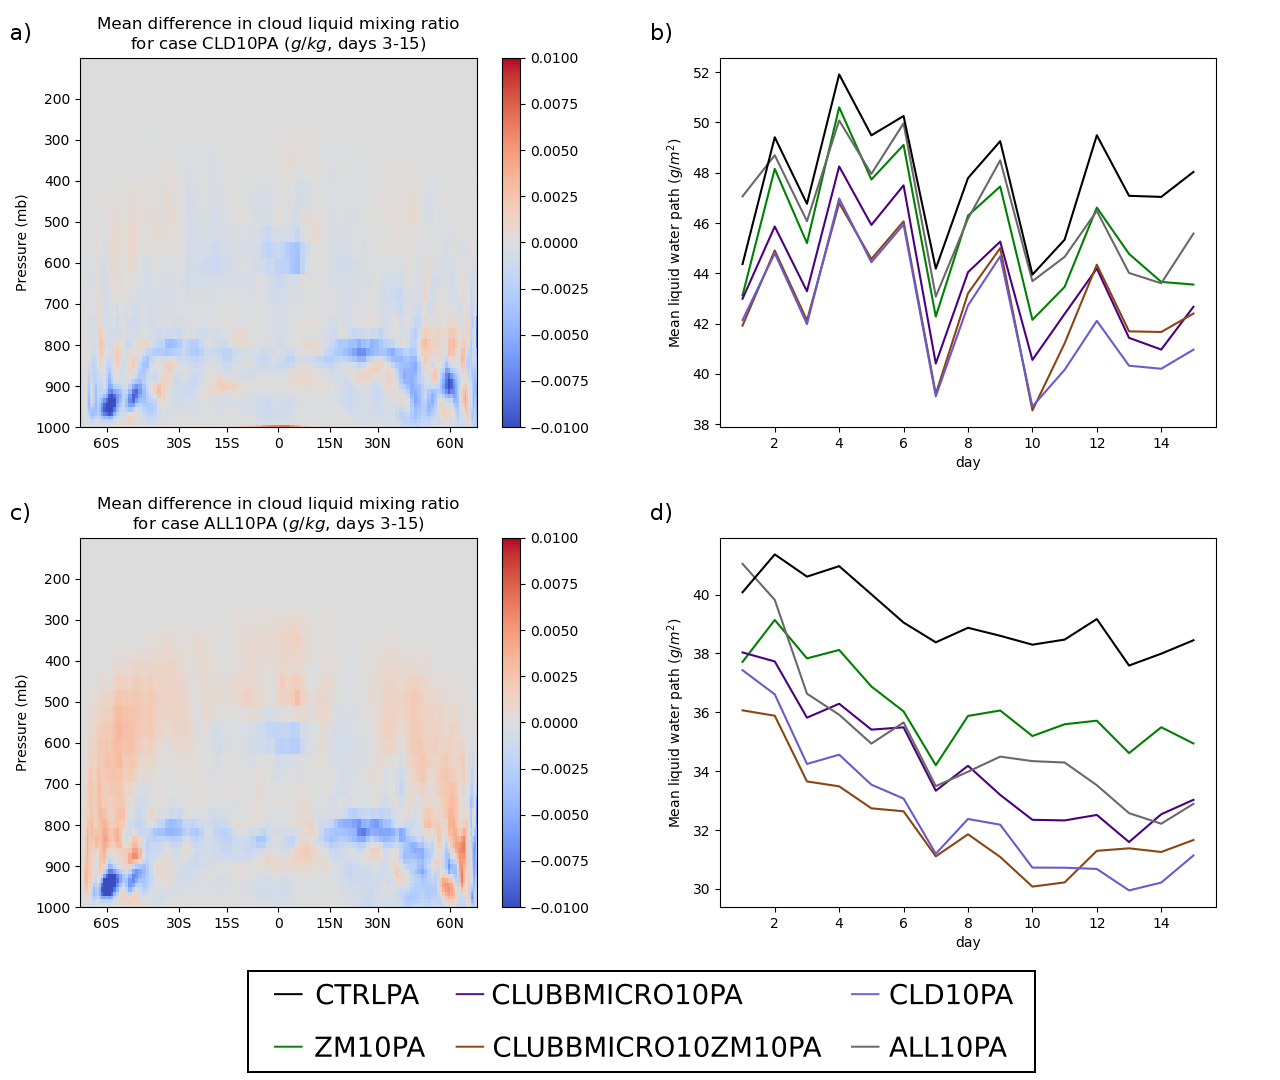
\includegraphics[width=5.5in]{Figure14.png}
    \caption{Left: Differences in zonal mean cloud liquid mixing ratio versus CTRLPA for a) CLD10PA and c) ALL10PA. Right: Daily liquid water path for prescribed aerosol substepped runs using b) a global mean, and d) a mean over low latitude grid points (\num{30}S--\num{30}N).}
    \label{fig:cldliq-pa}
\end{figure}

Other than this, ZM substepping accounts for very little of the differences between the CTRLPA and ALL10PA runs. There are small decreases in cloud fraction (not shown), but these are much weaker than the effect of increased dynamics-physics coupling frequency below \SI{700}{\millibar}, and weaker than the effect of a smaller CLUBB and MG2 time step above \SI{700}{\millibar}. The effect on shortwave cloud forcing, as seen in Figure \ref{fig:cld-frc-pa}, is thus also relatively small compared with the effect of changing the CLUBB and MG2 time step. The effect of ZM substepping on longwave cloud forcing may appear to be more significant, since the CLUBBMICRO10ZM10PA run has almost the same longwave cloud forcing as the ALL10PA run. However, the mechanism here is completely different; all runs where ZM is substepped, including CLUBBMICRO10ZM10PA, have a dramatically lowered ice water path (not shown). ALL10PA and CLUBBMICRO10PA, on the other hand, have an ice water path similar to the control, and so the decrease in longwave cloud forcing is instead attributable to decreased cloud fraction in these cases.

\begin{figure}
    \centering
    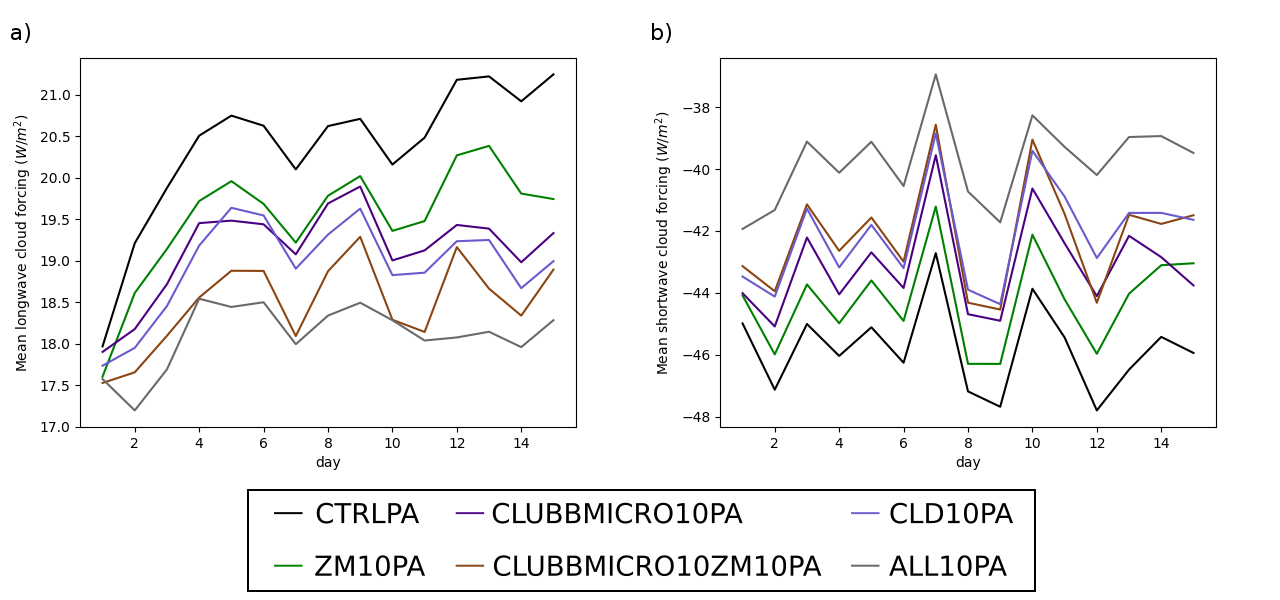
\includegraphics[width=5.5in]{Figure15.png}
    \caption{Daily global means of a) longwave cloud forcing and b) shortwave cloud forcing for prescribed aerosol substepped runs.}
    \label{fig:cld-frc-pa}
\end{figure}

\printendnotes

%
% ==========   Bibliography
%
%\nocite{*}   % include everything in the uwthesis.bib file
%\bibliographystyle{plain}
\printbibliography[heading=bibintoc]
%
% ==========   Appendices
%
\appendix
\raggedbottom\sloppy
 
% ========== Appendix A
 
\chapter{Where to find the files}


\vita{Blah
}


\end{document}
